\documentclass[oneside]{book}
\usepackage[a4paper, total={6in, 8in}]{geometry}
\usepackage[english]{babel}
\usepackage[utf8]{inputenc}
\usepackage[T1]{fontenc}
\usepackage{cancel}
\usepackage{amsmath}
\usepackage{amsfonts}
\usepackage{dsfont}
\usepackage{listings}
\usepackage{hyperref}
\usepackage{siunitx}
\usepackage{fancyhdr}
\usepackage{textcomp}
\usepackage{makecell}
\usepackage[font=small,labelfont=bf]{caption}
\usepackage{pdfpages}
\usepackage{multicol}
\usepackage[ruled,vlined]{algorithm2e}
\usepackage{soul}
\usepackage{mhchem}
\usepackage[toc, page]{appendix}
\usepackage{float}
\usepackage{wrapfig}
\usepackage{braket}
\usepackage{xcolor}
\usepackage{mathtools}
\usepackage{physics}
\usepackage{float}
\usepackage{subcaption}
\usepackage{tgbonum}


%Zotero Bibliography
%\usepackage{apacite}
%\addbibresource{bibliography.bib}


\pagestyle{fancy}
\fancyhf{}
\lhead{\rightmark}
\cfoot{\leftmark}
\rfoot{\thepage}

\setcounter{secnumdepth}{5}

\lstset{
    frame=tb, % draw a frame at the top and bottom of the code block
    tabsize=4, % tab space width
    showstringspaces=false, % don't mark spaces in strings
    numbers=none, % display line numbers on the left
    commentstyle=\color{green}, % comment color
    keywordstyle=\color{red}, % keyword color
    stringstyle=\color{blue}, % string color
    breaklines=true,
    postbreak=\mbox{\textcolor{green}{$\hookrightarrow$}\space}
}

\renewcommand{\lstlistingname}{}% Listing -> Algorithm
\renewcommand{\lstlistlistingname}{Algoritmi}% List of Listings -> List of Algorithms


\renewcommand*{\listalgorithmcfname}{}
\renewcommand*{\algorithmcfname}{}
\renewcommand*{\algorithmautorefname}{}
\renewcommand{\thealgocf}{}
\newcommand{\mathcolorbox}[2]{\colorbox{#1}{$\displaystyle #2$}}
\renewcommand{\familydefault}{\rmdefault}


\title{\Huge\textbf{Computational microbial genomics}}

\author{
  Giacomo Fantoni \\
  \small telegram: \href{https://t.me/GiacomoFantoni}{@GiacomoFantoni} \\[3pt]
\small Github: \href{https://github.com/giacThePhantom/computational-microbial-genomics}{https://github.com/giacThePhantom/computationl-microbial-genomics}}

\begin{document}
\maketitle
\tableofcontents

\chapter{Introduction}

\section{Microbes}
Microbes are defined as whatever is not visible at the human eye: bacteria cells' dimensions are in the order of micrometre, while viruses in the order of nanometre.
It is obvious how there is no visible part by eye.
This is particularly true for viruses: their dimension make them almost impossible to perceive by any other method than genomics.

	\subsection{Prevalence of microbes}
	We are living in a microbial world: more than $90\%$ of the biomass is composed of them and they are responsible for a great part of the biochemical cycle.
	Microbes can thrive in a variety of environment and according to some estimates they compose $10^{17}g$ of biomass.
	To put that in context the overall weight of the human species is three or four order of magnitude less.
	They also form the human microbiome, with important medical implication.

	\subsection{Difficulties in studying them}
	Of the predicted $30$ million species to exist only thousands can be cultured in isolation in the lab.
	There is a need to create a way to directly study and characterized samples taken from the environment.

\section{Genomics}
Once the genetic material is isolated and sequenced a huge amount of information needs to be interpreted.
The first sequenced gene was one of a bacteriophage.
Also the first complete genome wase one of a bacteriophage and is used by ILLUMINA as a control.
The first bacterial genome was published in $1995$ and was that of Haemophilus influenzae.
It has a dimension of $1.8Mb$ and sequencing took a year to complete.
The first archea was sequenced in $1996$.
In $1996$ the genome of S. cerevisiae has been sequenced and it was noticed that the genome shows a considerable amount of genetic redundancy.
The next step was to elucidate the biological functions of these genes.

	\subsection{Comparative genomics}
	Studying two different strains of the same organism difference in the genome can be linked to the difference in phenotype.

	\subsection{Metagenomics}
	Metagenomics is the study of the DNA from all the genomes in an environment.
	By sampling all of the DNA from a given environment, it is possible to study the presence of bacterial ecosystems, independent of the ability to culture bacterial in the lab.
	Large evolutionary radiation of bacterial lineages whose members are mostly uncultivated and only known through metagenomics and single cell sequencing have been described as nanobacterial.
	They have small genomes and lack several biosynthetic pathways and ribosomal proteins.

\section{Leveraging computational power}
Despite the advantages in DNA sequencing technology the sequencing of genomes has not progressed beyond clones on the order of the size of $\lambda$ because of the lack of sufficient computational approaches that would enable the efficient assembly of a large number of independent, random sequences into a single assembly.
When moving from low-throughput to high-throughput biology statistical power is needed: the genome of a bacterium must comprise all the DNA coding molecules present in the cell/
With millions of reads from NGS of an environmental sample, it is possible to get a complete overview of any complex micro biome with thousands of species.

	\subsection{Comparing low-throughput and high-throughput pipeline}
	In a low throughput pipeline to find the pathogenic agent for a novel outbreak a panel of reasonable putative causative agents is identified.
	Then one-by-one cultivation protocols to grow the agents from the infected tissue are performed.
	This is very time consuming.
	High-throughput instead sequences the full DNA repertoire of the sample and try to identify the pathogen by its genomic signature.

\graphicspath{{chapters/images/01/}}

\chapter{\emph{Escherichia Coli} general informations}
\section{\emph{E. coli} genomics}
\emph{Escherichia Coli} is a Gram-negative, facultative anaerobic, rodshaped, coliform bacterium, it pertains to the phylum of proteobacteria and to the family of Enterobacteriaceae. It can be grown easily and inexpensively. It has got genome with a length between 4.5 - 4.7 M bases, including about 4000-5000 genes, and about seven ribosomal RNA operons. Only the 38\% of the genes of K-12 (one of the most studied bacterial strains of \emph{E. coli}) were experimentally identified, overall 40-50\% of the genes are to date without a known function.
The original \emph{E. coli} strain K-12 was obtained from a stool sample of a
diphtheria patient in Palo Alto, CA in 1922.

\subsection{\emph{E. coli} long-term evolution experiment}
The \emph{E. coli} long-term evolution experiment led by Richard Lenski is one of the longest evolutionary experiments ever made (search "\textit{The Longest-Running Evolution Experiment}"). The experiment started on 24th February 1988, and since that moment 12 populations of \emph{E. coli} have been cultivated in the same environment. After each day (corresponding to the time of development of approximately 7 generations), a portion of bacteria from each flask was introduced in a new one, and let proliferating in it. Every 500 generation, it has been saved a sample of the bacteria of each flask, in order to track the evolutionary changes made. Today the experiment is on-going, and researchers reached approximately the 66000th generation. The study suggests a series of conclusions, to cyte "long-term adaptation to a fixed environment can be characterized by a rich and dynamic set of population genetic processes, in stark contrast to the evolutionary desert expected near a fitness optimum" (Good et al 2017). In fact, despite of the fixed environment, some bacteria developed the capacity to aerobically grow on citrate, which is unusual in \emph{E. coli} (around generation 31,000) and developed complex mutation patterns.


\subsection{\emph{E. coli} strains}
\emph{E. coli} could be found as commensal strains, pathogenic strains, or environmental strains. The pathogenic strains could pertein to these categories (which are not exclusive): enteropathogenic (EPEC), enteroinvasive (EIEC), enterotoxigenic (ETEC), diffusely adherent (DAEC), adherent invasive (AIEC), shiga-toxin producing (STEC), enteroaggregative(EAEC), extraintestinal pathogenic (ExPEC). Resistances to antibiotics make even more difficult the process of categorization of \emph{E. coli}.
In 2011 in Germany, an outbreak of Stx-EAEC was responsible of the death of some people. An efficient counter-measure was found by sequencing the genome of those bacteria.

Shigella is \emph{E. coli} with shiga toxin. It had been an issue for toxonomists.

Most of the genes are on plasmids, circular, additional to chromosome, and can be moved easily horizontally. Plasmids between different strains can be moved in enterobacteriacae, this doesn't happen normally in other families.
Some \emph{E. coli} strains are even capable of causing tumors in humans: for example, colibactin-positive \emph{\emph{E. coli}} can cause colon and rectal cancer, by creating mutations which are responsable of the of the cancer onset.

several antigens can be used by taxonomists to cathegorize \emph{E. coli} strains. In particular there are the O, H, K antigens, respectively related to the somatic, the flagella and the capsule. O antigens are 171, Ks are 80 and Hs are 56.

\subsection{PanPhlAn - strain detection and characterization}

Pangenome-based Phylogenomic Analysis (PanPhlAn) is a strain-level metagenomic profiling tool
for identifying the gene composition and in-vivo transcriptional activity of individual strains in metagenomic samples. PanPhlAn’s ability for strain-tracking and functional analysis of unknown pathogens makes it an efficient tool for culture-free infectious outbreak epidemiology and microbial population studies (\href{http://segatalab.cibio.unitn.it/tools/panphlan/}{PanPhlAn reference}). This tool was for example used to study the strain responsible of an outbreak in Germany in 2011. This strain was a shiga-toxigenic Escherichia coli (STEC), and the study was conducted by Loman and collegues in 2013.
This method outlasted the traditional one.


sequencing means generally to sequence everything, it's normally difficult where to find it, although in \emph{\emph{E. coli}} is quite easy to understand the provenience.
from all the world, populating diversity of \emph{\emph{E. coli}}, every time we sample we find points which are different from the reference genomes.
points overlapping are people living together and share bacterias


\subsection{Genomes of \emph{E. coli}}

In the genome of \emph{E. coli} strains, it is possible to distinguish:

\begin{itemize}
    \item \textbf{Core genome}: the set of all genes shared by all membrers of a bacterial species, it includes 1000 up to 3000 genes.
    \item \textbf{Accessory or dispensable genome}: the set of genes present in some but not all genomes within the same bacterial species. found on a single strain or in a subset of strains.
    \item \textbf{Pangenome}: core genome + accessory genome. set of all the genes foundable in the species strains. It is said to be \textit{\textbf{"closed"}} when pangenome size tends to a maximum as number of genomes increases, instead it is \textit{\textbf{"open"}} when pangenome keeps increasing as you add new genomes
\end{itemize}


Sequencing more organism of the same species means to lower the amount of genes in the core genome and augment the numer of those in the pan-genome (figure \ref{corepangenome}).
Because of technical problems the probability of getting a gene and not forget it is different from 0, so why probably the sequencing of other genomes would lead technically to a plummet to 0 of the pangenome. With some mathematical formulations we can predict a more probable plateau (Rasko David 2008).

% \begin{figure}[h]
% \caption{Core- and pan- genome of \emph{E. coli}}\label{corepangenome}
% \centering
% 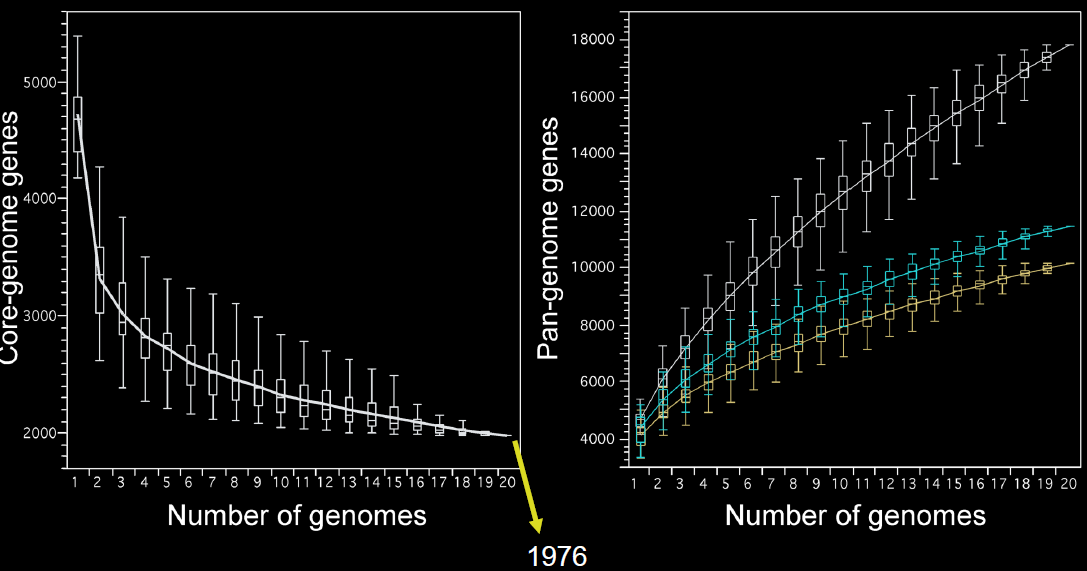
\includegraphics[width=0.6\textwidth]{EcoliCorePanGenome}
% \end{figure}


% \begin{figure}[h]
% \caption{It can be seen that 51\% of the genes are strain specific, and the other are shared between 2 to 20.  of \emph{E. coli}}
% \centering
% 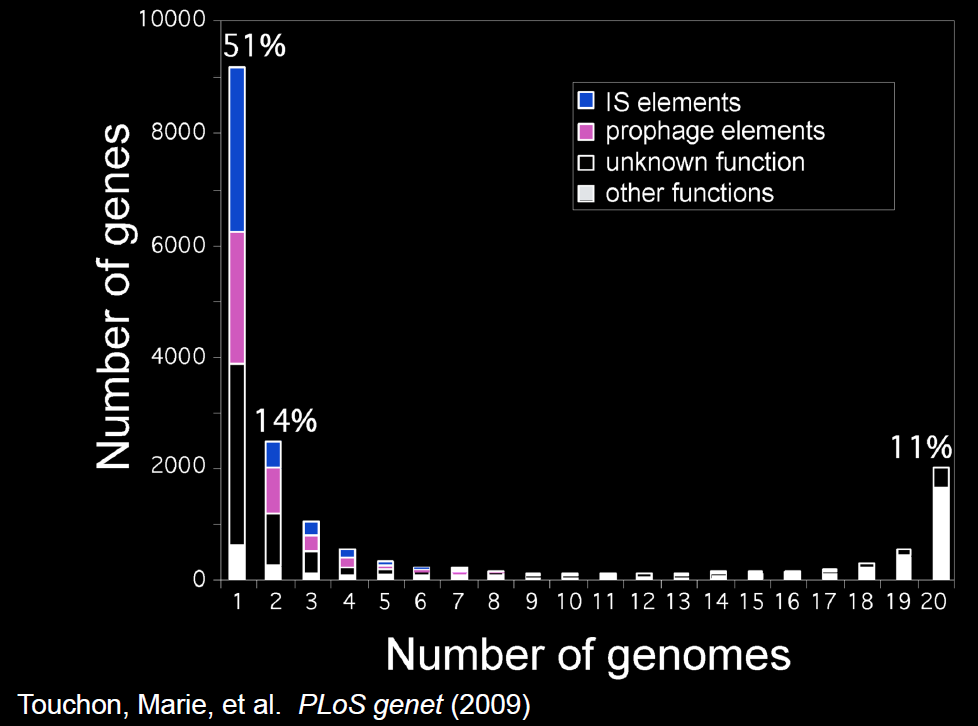
\includegraphics[width=0.6\textwidth]{genesSharedDifferentGenomes}
% \end{figure}


% \begin{figure}[h]
% \caption{A different definition of orthologous genes can modify the number of pan genes of a species. }
% \centering
% 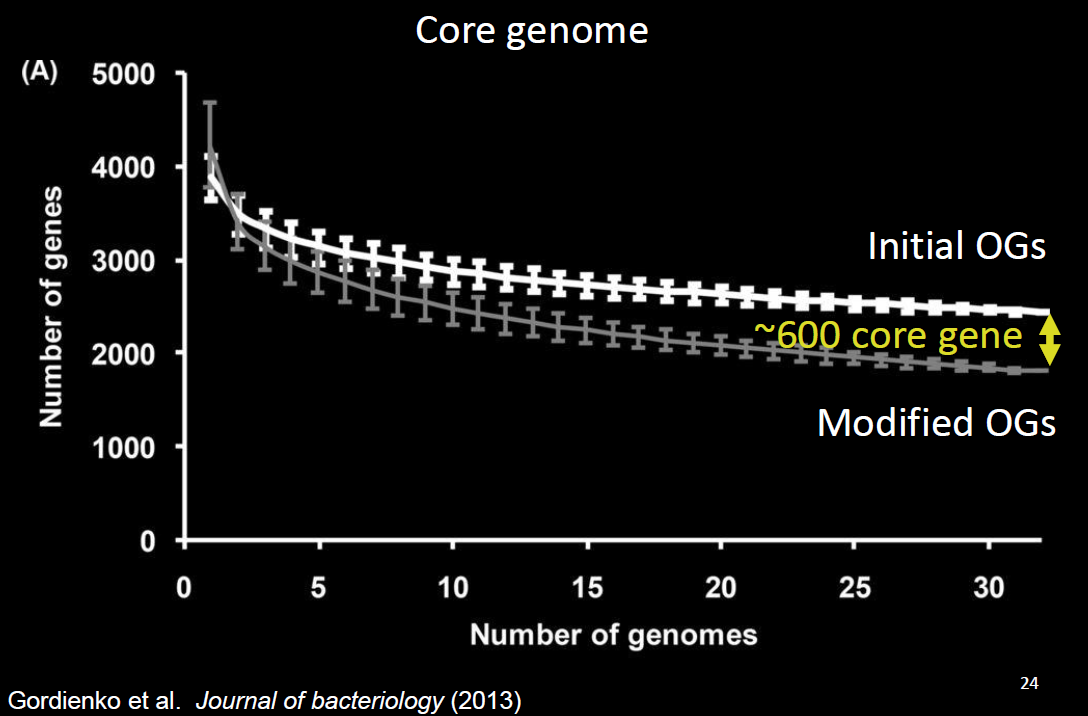
\includegraphics[width=0.6\textwidth]{orthologGenes}
% \end{figure}


% \begin{figure}[h]
% \caption{we predict a core genome size of 3079 genes for extraintestinal pathogenic \emph{E. coli}}
% \centering
% 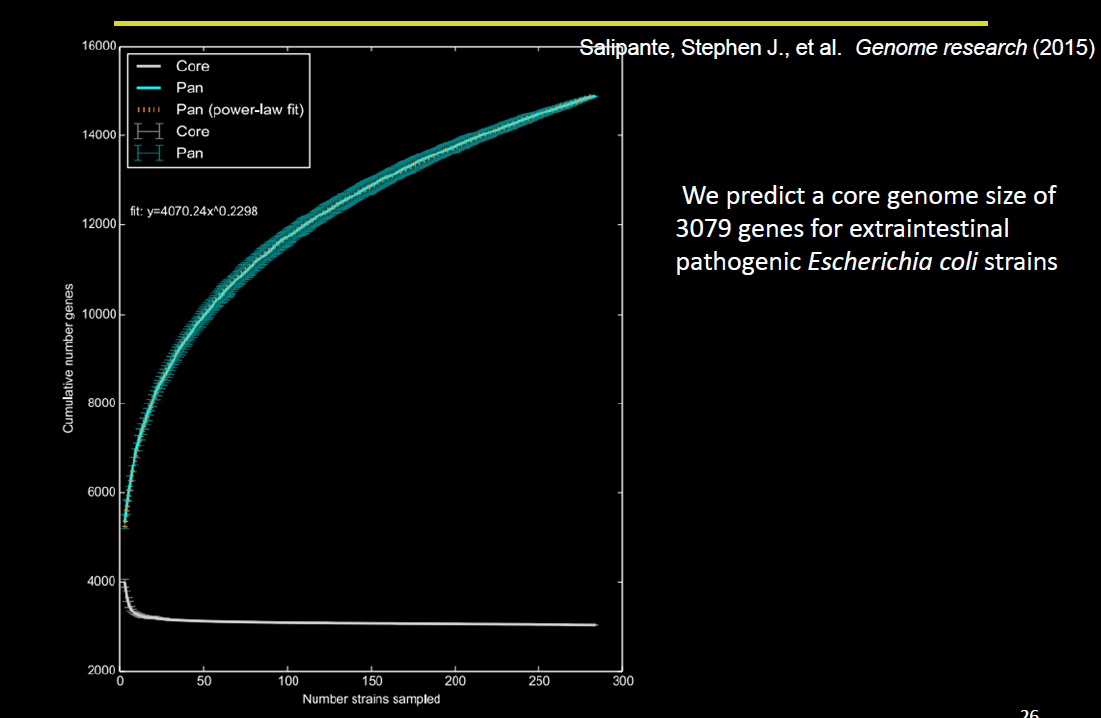
\includegraphics[width=0.6\textwidth]{coreGenomePredict}
% \end{figure}

each \emph{E. Coli} genome contains in a balanced way genes of the core genome and of the pan genome, for a total amount of genes correspondant to about 4700 genes (figure \ref{balancepancore}). Core genomes' genes are responsible of some basic cellular functionalities and utilities to survive environent, while instead elements of the pangenome are quite usually specific to the single strains, they are not always functionally well known.


% \begin{figure}[h]
% \caption{Balance between genes of the core- and of the pan-genome}\label{balancepancore}
% \centering
% 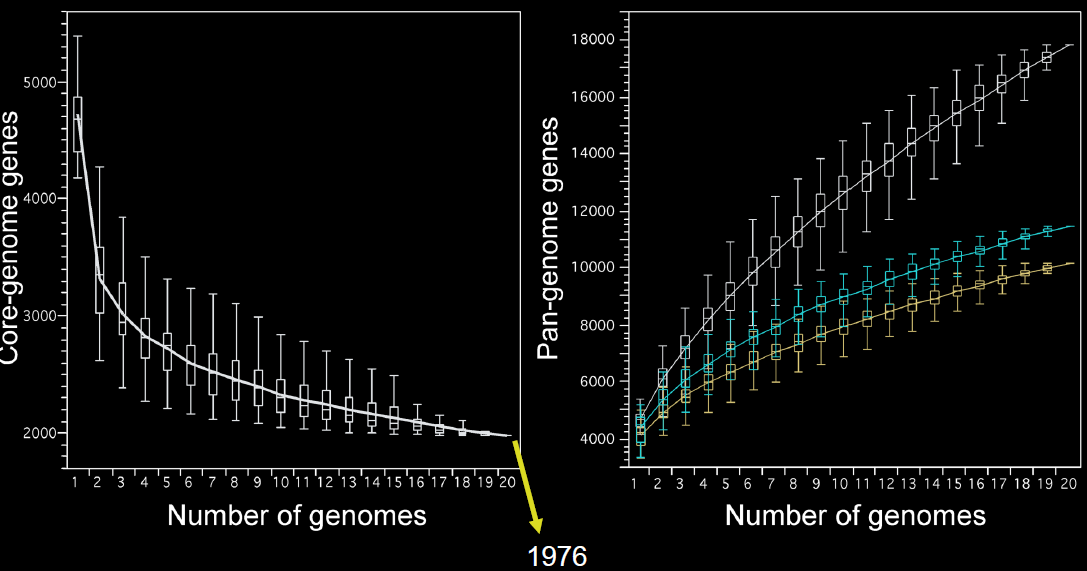
\includegraphics[width=8cm]{corePanGenEcoli}
% \end{figure}


ratios of the pan-genome and the core-genome are not equal in other
organisms behave differently.

\graphicspath{{chapters/images/03/}}

\chapter{NGS principles (second gen. sequencing) - From Sanger to third gen sequencing}

\begin{figure}[h]
\caption{}
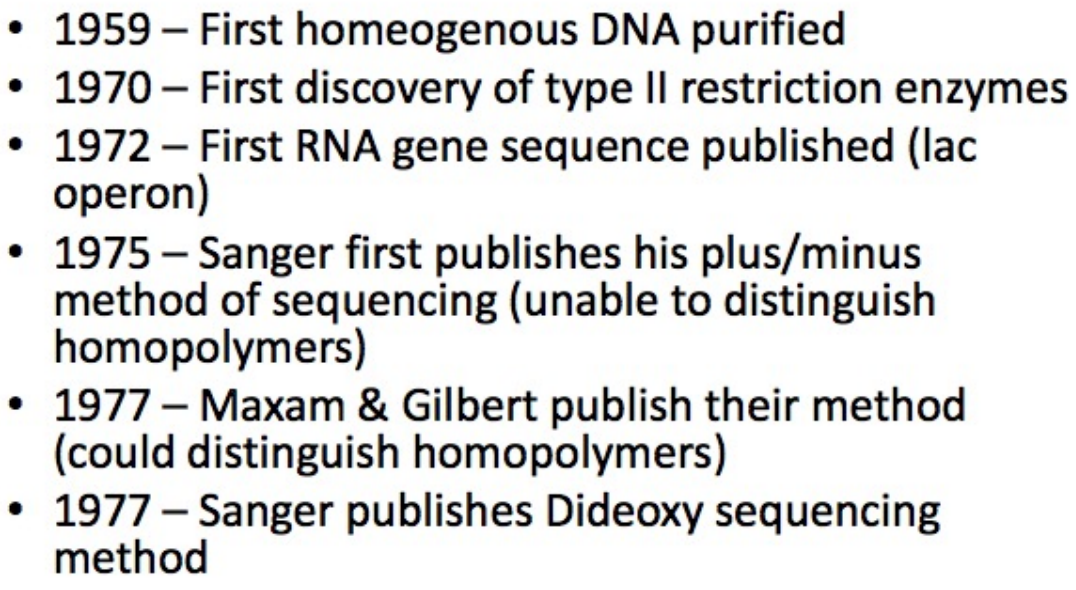
\includegraphics[width=0.6\textwidth]{history-seq}
\label{discoveries-sequencing}
\end{figure}

NGS stands for \textbf{\textit{Next Generation Sequencing}}, and it represents the method of sequencing most used nowadays. Before that, a series of other discoveries were done, elencated in the figure \ref{discoveries-sequencing}.

\section{History of Sequencing}
\subsection{Progresses of sequencing}
As the time passes, the cost of sequencing the DNA is diminishing. The rate of decrease actually is higher than the one predicted by the \textbf{Moore's Law}, \textit{"Democratization of sequencing"} is seen nowadays, because of the costs lowering. After the Human genome project, several other animals and plants' genomes were sequenced.

\begin{figure}[h]
\caption{}
\centering
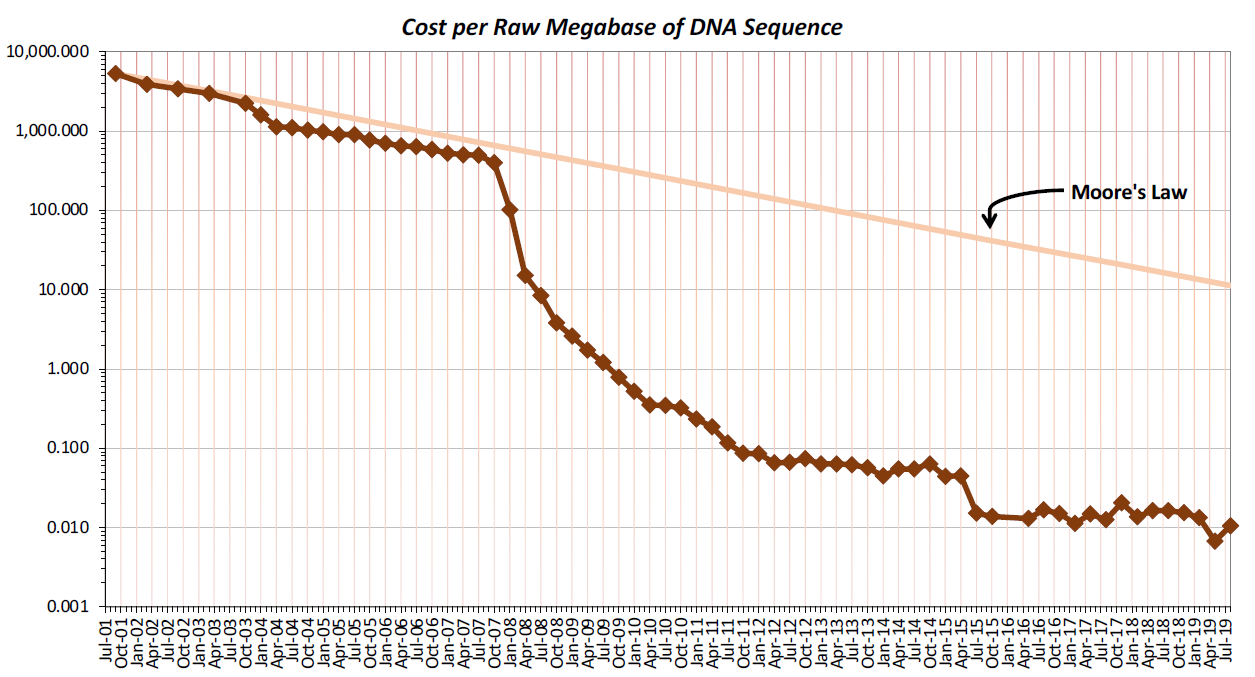
\includegraphics[width=0.6\textwidth]{sequencingCost}
\label{Moore's law graph}
\end{figure}

The methods of sequencing actually can be grouped in three \textbf{groups}, that are:

\begin{itemize}
	\item \textbf{Chemical degradation} of DNA: it includes the method of Maxam-Gilbert
	\item \textbf{Sequencing by synthesis (“SBS”)} which is the most common approach and the first to be developed. It uses DNA polymerases in primer extension reactions Illumina, Pacific Bioscences, Ion Torren and 454
	\item \textbf{Ligation-based}: sequencing using short probes that hybridize to the template, the technologies perteining to this class are SOLiD, Complete Genomics
	\item \textbf{Other:} Nanopores
\end{itemize}

\subsection{The Chain Terminators}

\begin{figure}[H]
    \centering
    \begin{subfigure}[b]{0.49\textwidth}
        \centering
        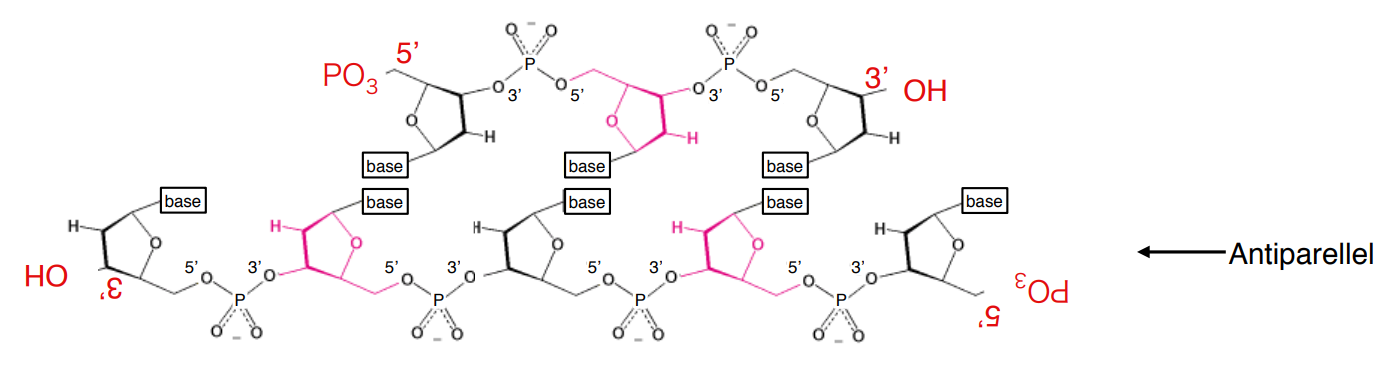
\includegraphics[width=\textwidth]{DNA-molecule}
        \caption{Normal DNA molecule, with oxydrilic group ligated to $3'$-ends}
        \label{normalDNAaddition}
    \end{subfigure}
    \hfill
    \begin{subfigure}[b]{0.49\textwidth}
        \centering
        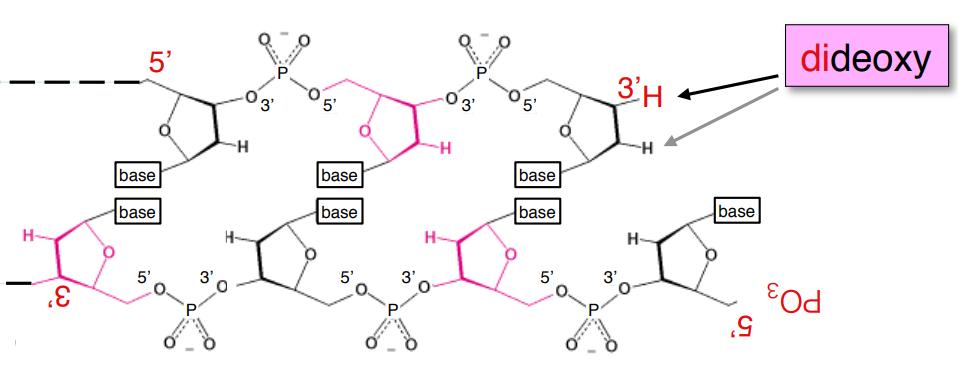
\includegraphics[width=\textwidth]{chain-term}
        \caption{Figure representing the difference between a normal DNA chain and one with chain terminators}
        \label{ChainTerm}
    \end{subfigure}
    \caption{Normal DNA synthesys \textit{vs} Chain terminators}
\end{figure}


Normally, the addition of new nucleotides to a generated molecule of DNA happens with the $3'$-end of the nucleotide chain (figure \ref{normalDNAaddition}). Chain terminators are dideoxy nucleotides, ddNTPs, that cannot be further extended. These nucleotides aren't able to add a new nucleotide on the $3'$-end, as they have not the needed oxydrilic group (figure \ref{ChainTerm}).

\subsection{Sanger method: the first one}

\begin{figure}[h]
\caption{The \textit{Sanger}'s method process}
\centering
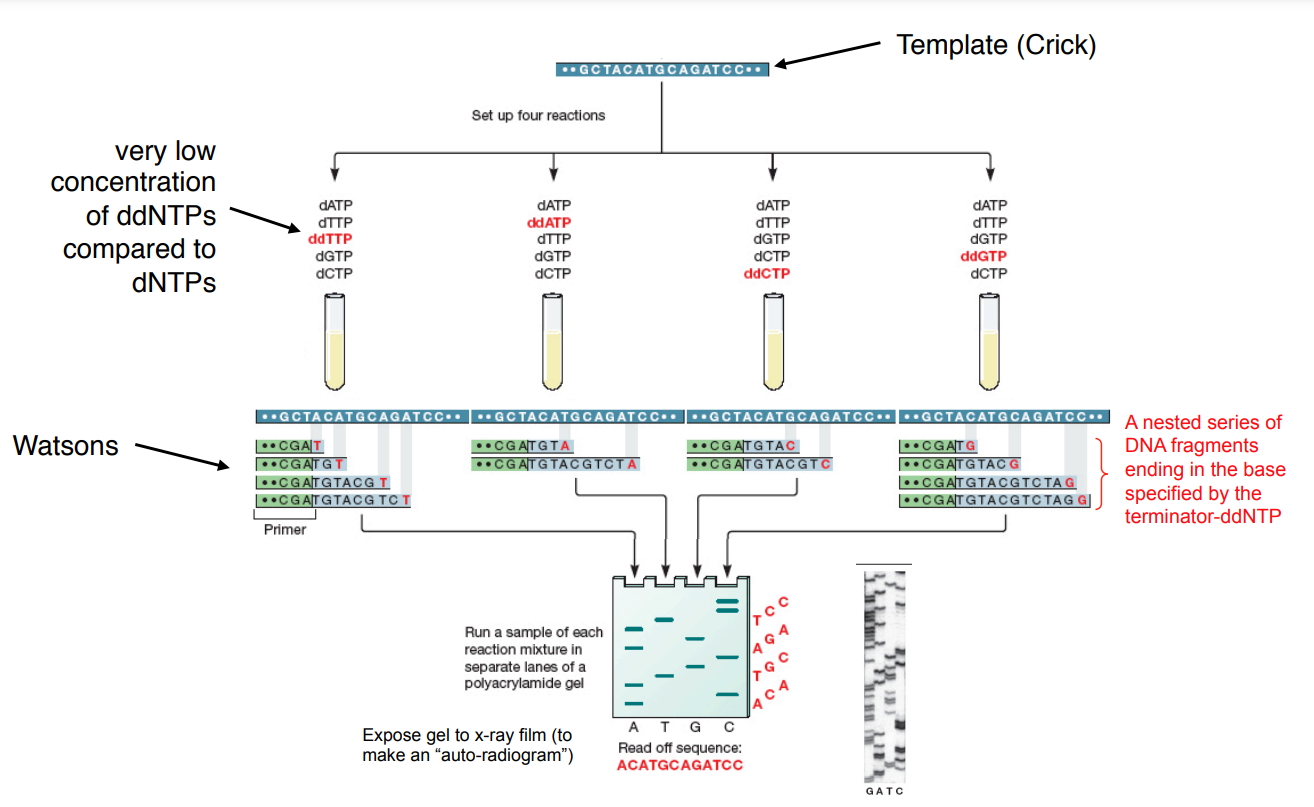
\includegraphics[width=\textwidth]{Sanger}
\label{Sanger}
\end{figure}

The first method ever used to sequence DNA was designed by Frederick Sanger. The Sanger manual sequencing system consists in an \textit{in vitro} process, which is described in figure \ref{Sanger}, also named as \textit{"primer extension"} method. It is performed over a single-filament DNA sample, and it uses the chain terminators nucleotides, a type for each nucleobase: ddATP, ddGTP, ddTTP, ddCTP.

The reaction is done inside four different reactions tubes, each containing the sample DNA to be reproduced, a DNA polymerase, the normal nucleotides and one of the four possible chain terminator. The chain terminators are marked with sulfur-35, a radioactive atom. In each tube, the corresponding dideoxy-nucleotide was used with a concentration 10 times lower than the other "normal" nucleotides.

From the polymerization reactions, several molecules of DNA were produced, with different length: each replicative cycle is in fact terminated after the addition of a chain terminator nucleotide.

To reconstruct the initial DNA sequence, a long PAGE gel was prepeared, with high concentration of urea ($6 - 7 M$) to avoid the coiling of the DNA single-filaments. To run the gel, high voltages were required and it had to be higly resolutive, as DNA's fragments are different only for a nucleotide. It was needed to do an auto-radiography of the gel in order to see the bands, in order to evidentiate the fosphorescent signals.

To read the sequence you have to start from the shortest fragments, at the end of the gel, and carefully go up along the gel, looking for the first presence of a band in one of the four runs. \\

\textbf{Past procedures: }In the past, the Klenow's fragment (part of the $1^{st}$ DNA polymerase) was used to perform the Sanger method, and the DNA to be sequenced was inserted inside the genome of an M13 phage.


\subsubsection{Automatic sequencing}
It does not use the radioactive signals, instead it uses fluorescent proteins. Several versions were developed after modifications of the Sanger method, in this order:

\begin{enumerate}
	\item fluorescent primers marked with a single fluorochrome.
	\item four aliquotes of the same primer were used marked with four different fluorochromes, able to emit different fluorescences.
	\item four different fluorochromes were used to mark the single ddNTPs
\end{enumerate}

Thanks to the use of 4 different fluorochromes, it was possible to use a single electrophoretic lane to carry the sequencing reaction. For this type of sequencing also, a cyclic replicative reaction was performed, with this procedure, made possible by using a thermal cycler:

\begin{enumerate}
	\item \textbf{Denaturation at $95$°C} of the DNA to be sequences
	\item \textbf{Annealing at $50-70$°C} of the primer specific to one of the two filaments
	\item \textbf{Extension at $72$°C} by using a \textit{Taq}-polymerase. The use of the Taq-polymerase makes it possible to avoid the formation of coiled structures in the DNA molecule to be sequenced.
\end{enumerate}

Traditionally, also in this type of sequencing it is used a long PAGE gel, as the Sanger's one, but with a great difference: all the ddNTPs are inserted in the same electrophoretic run, and after it, it is not needed an auto-radiography. Fluorescence, instead, can be triggered simply by irradiating the DNA molecules synthesyzed, which produce different fluorescences with different wavelengths.

\begin{figure}[h]
\caption{}
\centering
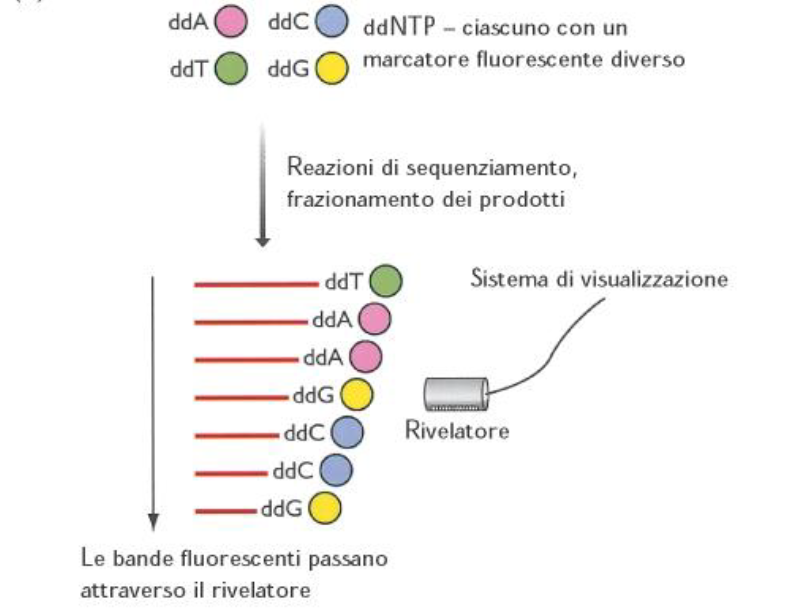
\includegraphics[width=0.8\textwidth]{automaticSang}
\label{}
\end{figure}


More usefully, this sequencing method is performed by using a capillar, filled with a synthetic polymer, with the same function of polyacrillamide.

At the end of the analysis, it is produced an electropherogram, with a color depicting the probability of each nytrogen base in each position. The production of the electropherogram is made better thanks to algorithms to boost signal/noise ratio, to correct the dye-effects, and other effects that generate systemic errors. %TODO dye-effects

\begin{figure}[h]
\caption{}
\centering
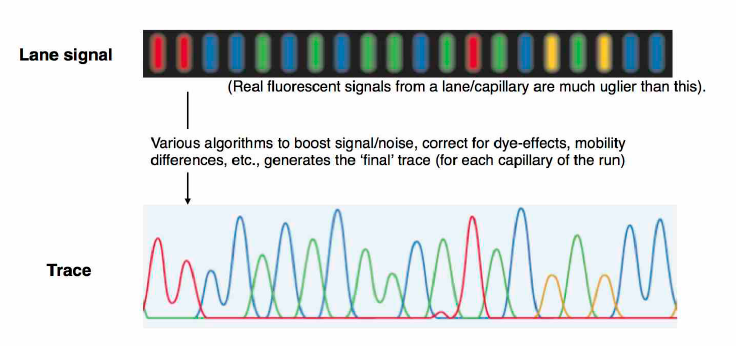
\includegraphics[width=0.8\textwidth]{elettroferogramma}
\label{}
\end{figure}

\begin{figure}[h]
\caption{The implementation of capillary sequencing machines gave the possiblity to make more runs than with the others. A $\tilde 1000$ fold productivity increase was allowed}
\centering
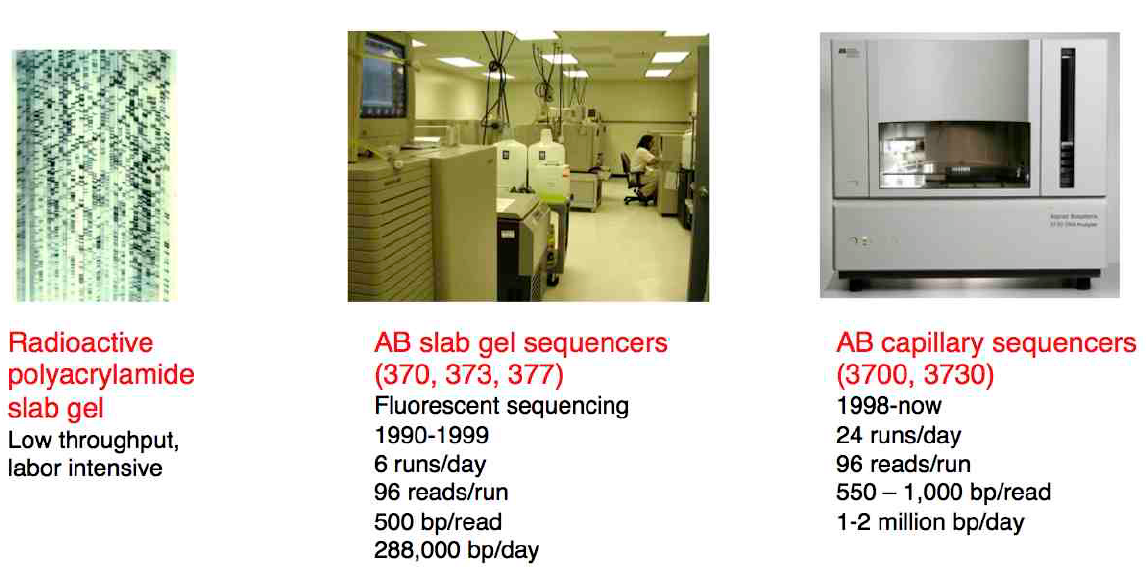
\includegraphics[width=0.8\textwidth]{progressSangerMachines}
\label{}
\end{figure}

Regarding the Sanger machines in use, the upgrades viewable in figure \ref{progressSangerMachines}. Based on the same technology, new machines were developed and it was obtained a $\tilde 1000$ fold improvement.
\\
When talking about the \textbf{human projec}t, it is important to specify that most of the job was done by using the Sanger automatic sequencing method.


\section{Development of Sequencing Machines}
The way you can get to the point could be different based on technology and the wanted output, comprised quality.

SOLID gave only $35$-$75$ sequenced bases, and it is not used anymore; Sanger sequencing, the capillary, can give up to 1000 read length, with a low output; on MINION it was possible to sequence an entire genome of \textit{E. coli}
A pletora of sequence machines are available today. None of the machines are able to sequence DNA from a sample of blood, some things have to be done. Nowadays \underline{machines producing bigger outputs of short reads are prefeared}.

\begin{figure}[H]
\caption{It can be noticed how recent developments had the scope of increasing the output data}
\centering
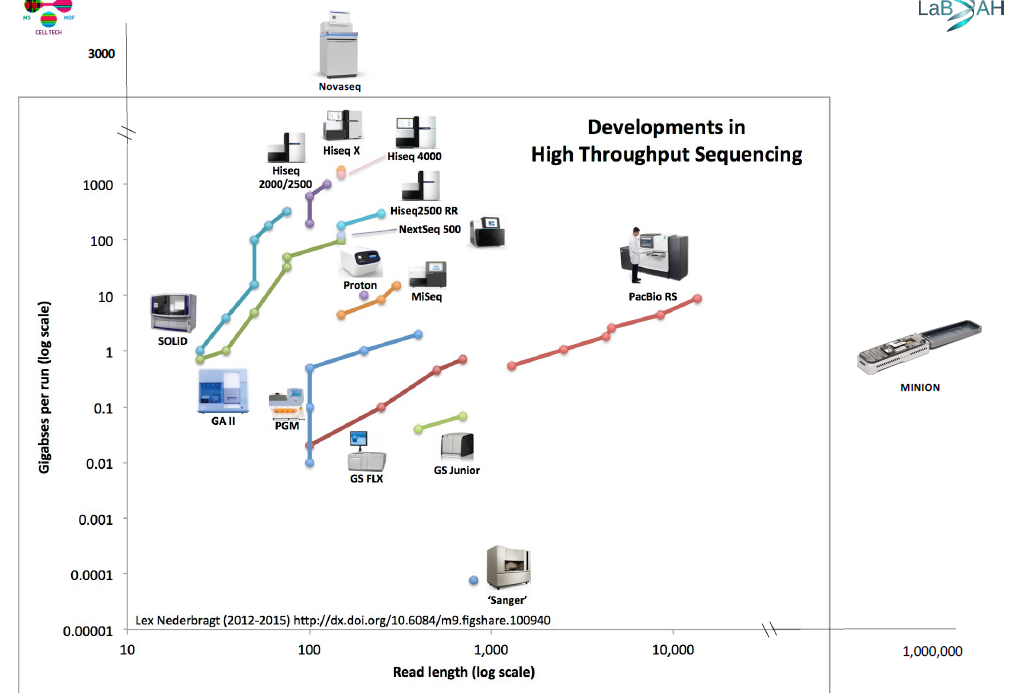
\includegraphics[width=1\textwidth]{sequencingMachines}
\label{}
\end{figure}

At the top of the market nowadays there are ILLUMINA machines, that use sequencing by synthesis method, NovaSeq is the biggest one. They need to amplify the signal through clusters formation.

\begin{figure}[H]
\caption{}
\centering
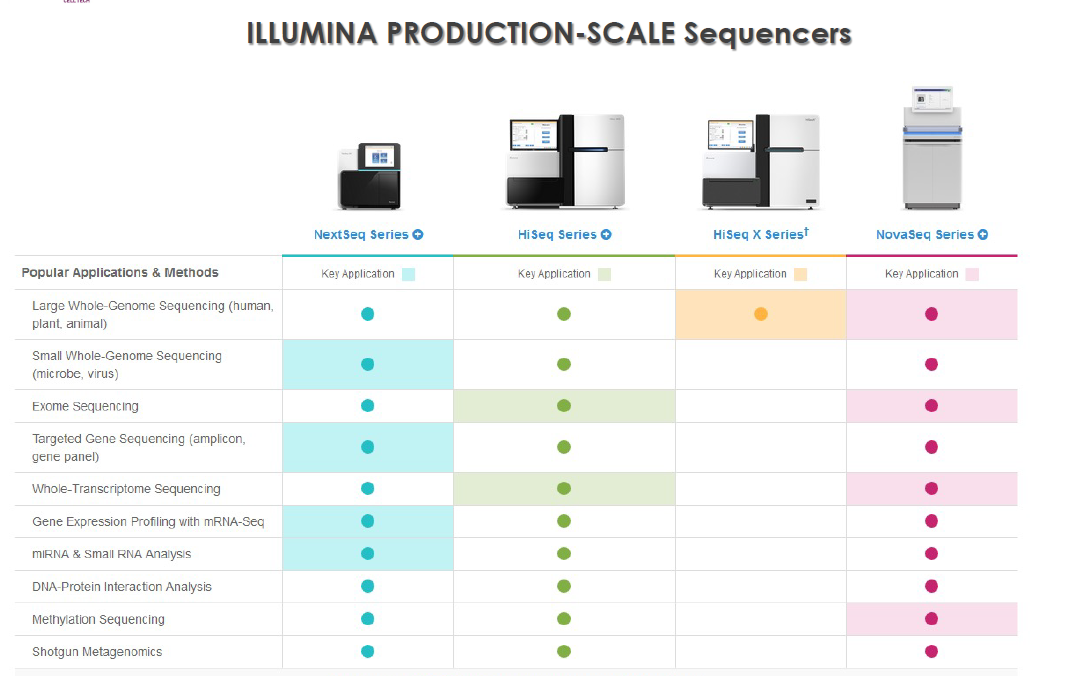
\includegraphics[width=0.8\textwidth]{sequencingMachinesIllumina}
\label{}
\end{figure}

\section{Next Generation Sequencing NGS}

The NGS protocol requires $3$ steps, that are:

\begin{enumerate}
	\item \textbf{Sample preparation}: series of fragments added
	\item \textbf{Clonal amplification}: which is is needed to replicate fragments attached to the solid surfaces, since machines are not sensible to single molecules
	\item \textbf{Sequencing}: ILLUMINA sequencing is one of the techniques used to obtain sequence data nowadays
\end{enumerate}

Tools pertaining to the $3^{rd}$ generation are those that permit to read a molecule without replicating it.

\subsection{Fragments/Library preparation}
Most of the sequences sequenced are fragmented in short read sequences, since most of the machines today used aren't able to sequence reads longer than some hundreds of nucleotides.

% Fragmantation is so required to generate shorter filaments from the sequences. In the case of mRNA (cDNA libraries) the fragmentation process is not needed, as the lengths are already short enough.

The fragments obtained have to be prepeared for the sequencing process, through a process called \textbf{tagmentation}. The obtained fragments are shown in the figure. Those fragments are provided with one or two indexes, called also barcodes, two sequencing primer binding sites and regions complementary to the oligonucleotides present in the chamber (see in Clonal amplification chapter). The fragments' length has to be checked, depending on the scope of the process. Indexes are needed to run sequencing process on multiple samples, they are needed to distinguish those; when they are two, they permit to distinguisch also the 2 types of sequencing that are performed, forward and reverse.

P5 and P7 are the oligos needed to attach fragments to ILLUMINA sequencing machines.

\begin{figure}[h]
\caption{Figure representing the a good prepeared fragment, it has two indexes, two sequencing primer binding sites and regions complementary to the oligonucleotides present in the chamber}
\centering
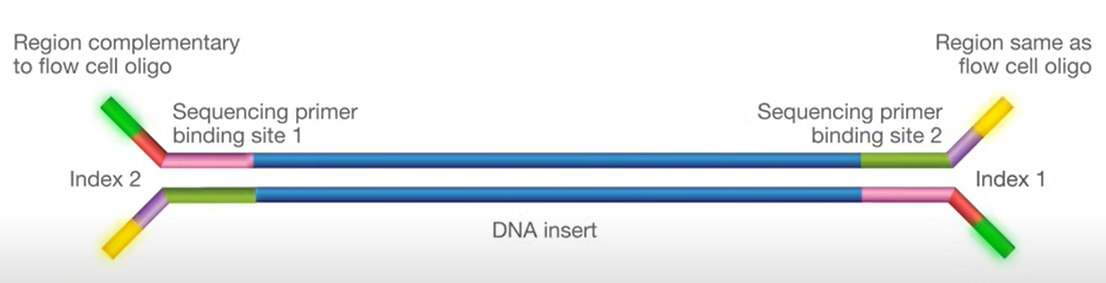
\includegraphics[width=0.8\textwidth]{tagmentedFragments}
\label{}
\end{figure}

%what is a good fragment? %TODO

\subsection{Clonal amplification and ILLUMINA sequencing procedure}

\begin{figure}[h]
\caption{}
\centering
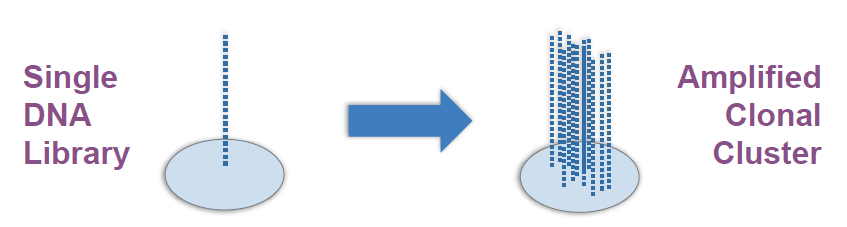
\includegraphics[width=0.6\textwidth]{clusterAmplification}
\label{clusters}
\end{figure}

Clonal amplification are necessary to amplify the signal from each single fragment.
ILLUMINA machines make use of clusters to sequence DNA. Clusters are a group of DNA
strands positioned closely together and generated from a single DNA filament. Generally, Each cluster represents thousands of copies of the same DNA strand in a 1–2 micron spot (figure \ref{clusters}).

\begin{figure}[h]
\caption{}
\centering
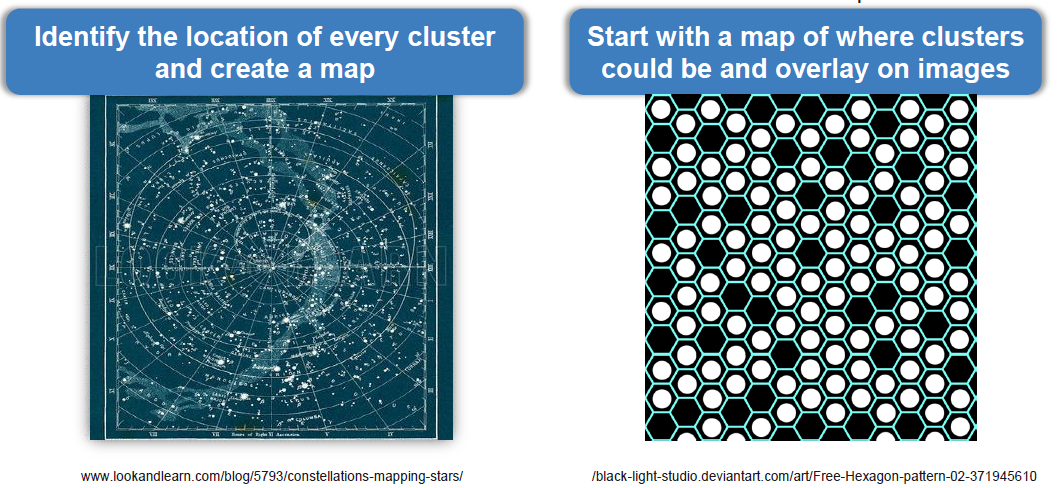
\includegraphics[width=0.8\textwidth]{rigidGeneration}
\label{rigid}
\end{figure}

On patterned flow cells, the clusters' formation location could be known or not, in the first case it is said that there is a "Rigid registration" (figure \ref{rigid}).\\


ILLUMINA sequencers normally use slides of glass, named flow cells, and the fragments to be sequenced are able to flow over the channels. The temperature inside the cells can be changed to produce ligations or separations. The surface of the cells is functionalized with a series of oligos complementary to library adapters.

Two kids of flow cells, the \textit{patterned} flow cell permits to create clusters in specific positions, inside nanowalls, contrarily to \textit{Random Flow Cell} which instead have randomly positioned clusters.
\begin{figure}[h]
\caption{}
\centering
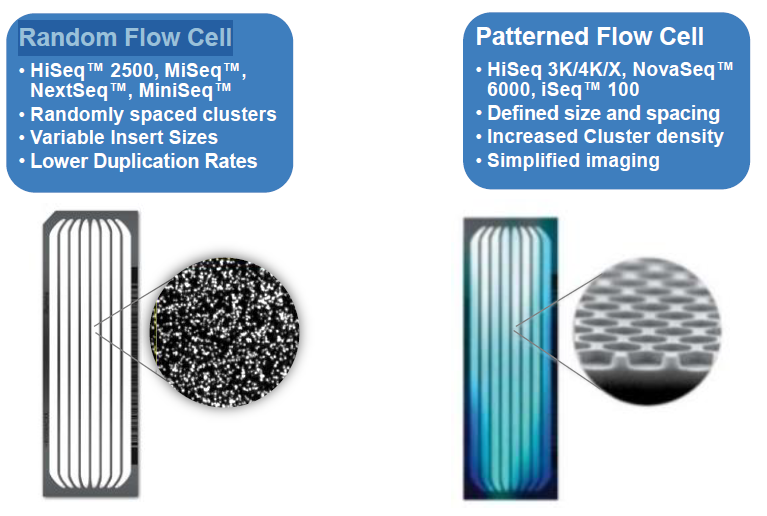
\includegraphics[width=0.6\textwidth]{randomPatternCells}
\label{}
\end{figure}
\\

Once the fragments are made flow over the chambers, they can bind only to p5 or p7 (ILLUMINA oligos), the two oligos functionalizing the plate. Once the fragments are attached to the surface, using temperature and solvents flows you can control the sequencing process. To see the entire procedure:
(procedure on Youtube: \href{https://www.youtube.com/watch?v=womKfikWlxM}{video about ILLUMINA sequencing}). In the video, it is shown the two index sequencing process.
\\
\\


\begin{figure}[H]
    \centering

    \begin{subfigure}[b]{0.39\textwidth}
        \centering
        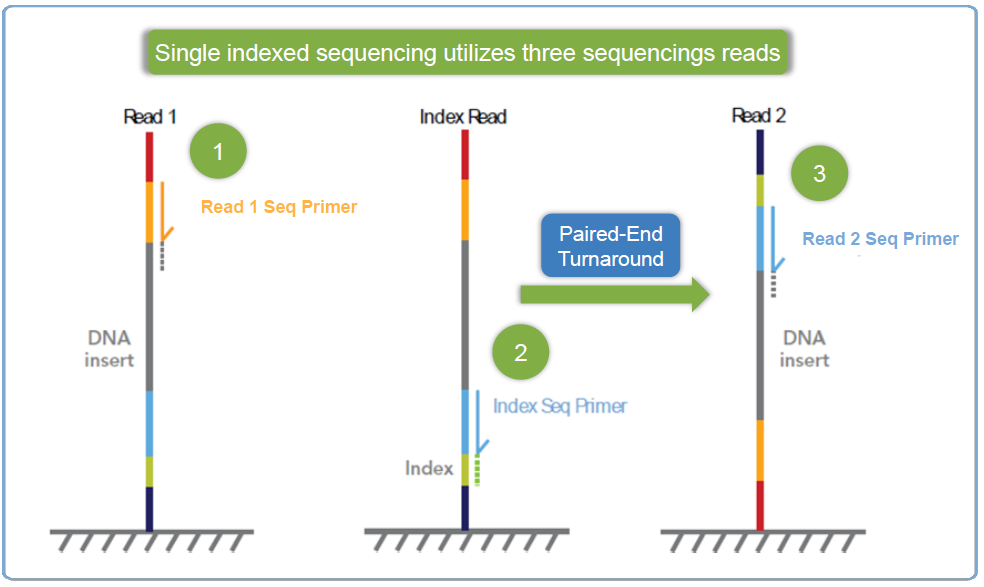
\includegraphics[width=\textwidth]{singleIndex}
        \caption{single index}
    \end{subfigure}
    \hfill
    \begin{subfigure}[b]{0.60\textwidth}
        \centering
        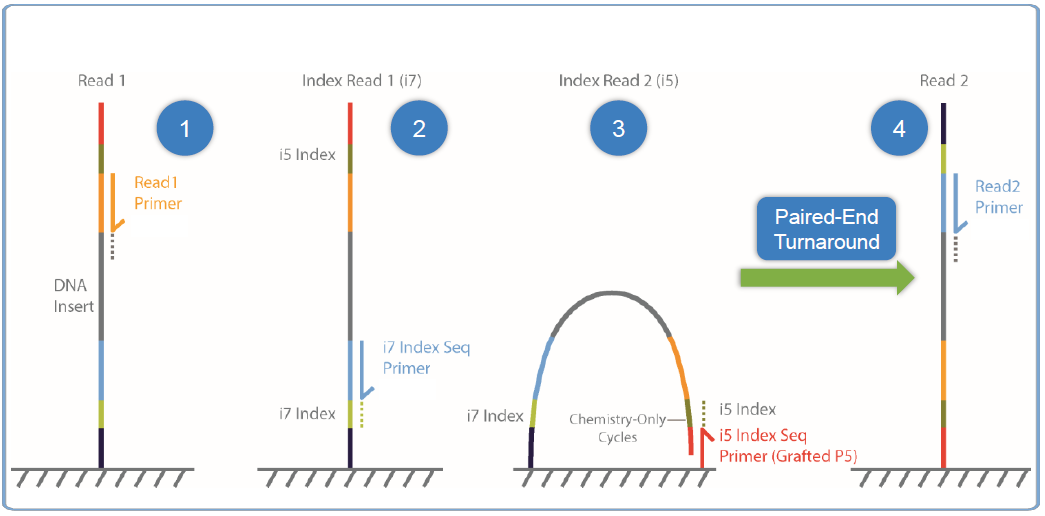
\includegraphics[width=\textwidth]{doubleIndex}
        \caption{double index}
    \end{subfigure}
    \caption{Single/double index for ILLUMINA sequencing}
    \label{singDoubInd}
\end{figure}

With 1 and 2 indexes the sequencing process actually differs, as shown in figure \ref{singDoubInd}


\begin{figure}[H]
\caption{}
\centering
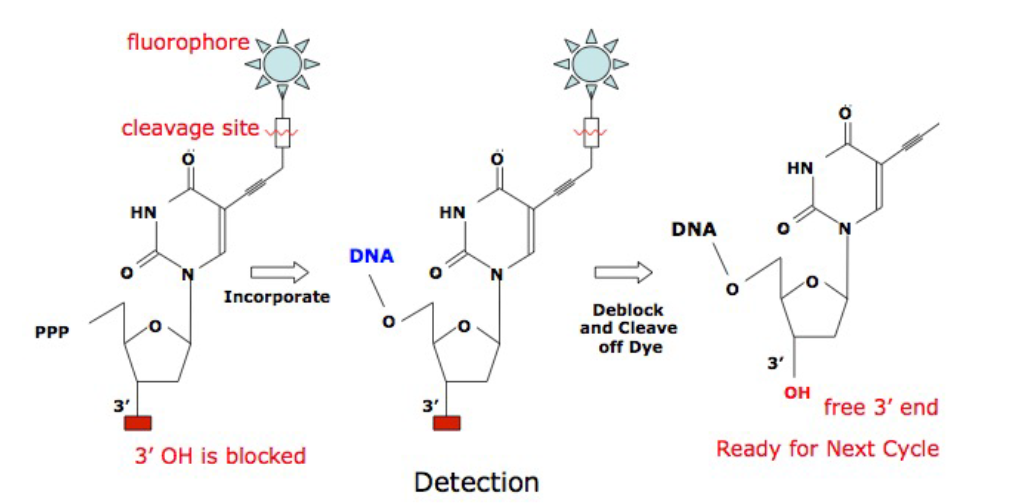
\includegraphics[width=0.7\textwidth]{ILLUMINArev}
\label{ILLUMINArev}
\end{figure}

To perform the sequencing process, ILLUMINA machines utilize \textit{reversible terminators} (figure \ref{ILLUMINArev}). They permit a real time analysis of the sequencing by synthesys reaction, and because of this they are different from the Sanger method. Fluorophores are reversible, they can be cleaved to eliminate the light signal.

\begin{figure}[h]
\caption{}
\centering
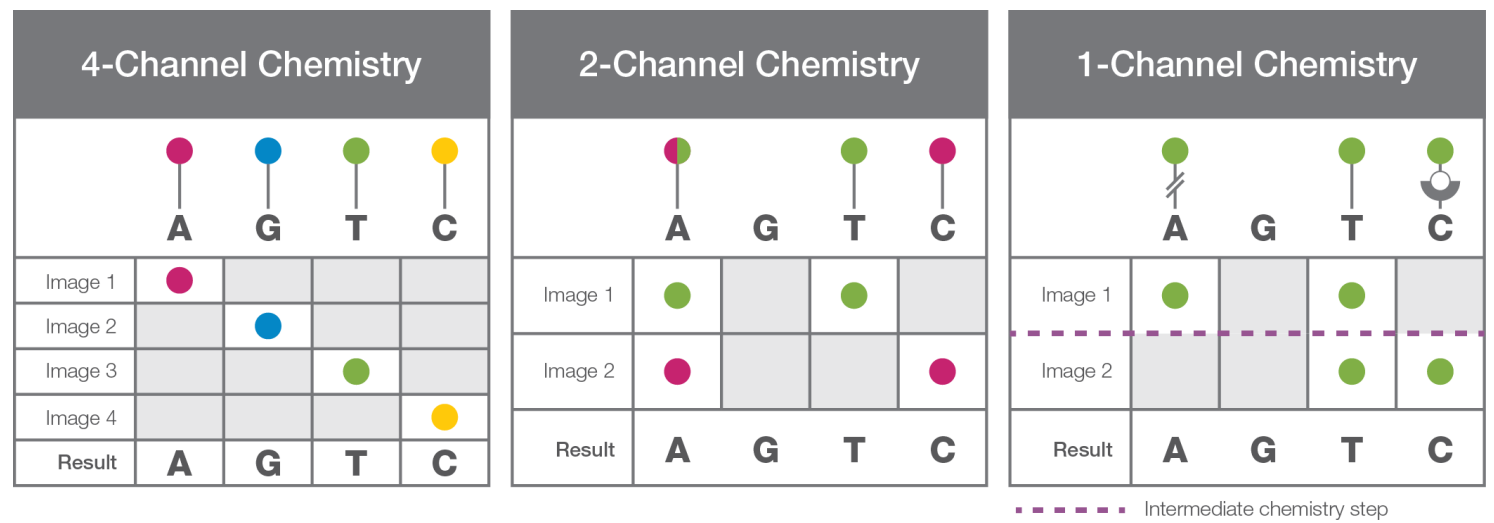
\includegraphics[width=0.8\textwidth]{ChannelILLUMINA}
\label{ChannelILLUMINA}
\end{figure}

To perform their activity, ILLUMINA sequencers could be of 3 different types: 4-Channel, 2-Channel or 1-Channel, depending on the number of fluorescent molecules used. In the case of the 4-Channel technology, 4 images are taken in each cycle, and each  cluster appears in only one of four images \ref{ChannelILLUMINA}. 2-Channel technique is used by some sequencing machines, like NextSeq 550, MiniSeq, NovaSeq 6000\\

4-Colors base calling
is needed to to make
the true signal the purest, and after, The base with the highest intensity becomes the called base for that cluster. In the case no base is clearly related to a position, \textit{N} is the result.


The reading process could be done in two ways: through single reads, on a single extreme of the fragments, of paired-end, on both the extremes. The second one in particular gives structural and 2 sequence  informations.


\subsection{Pacific Bioscience (PacBio)}
the long DNA filement to be sequenced is attached to a polymerase, over the surface of a SMRT (Single Molecule Real Time) cell. This cell is really small, and at each nucleation process a light signal is emitted. The produced light is not able to get out of the walls, and its duration is extremely restricted. Sequencing, also in this case, is made by sequencing, and the main advantage consists in the possiblity of sequencing really big DNA molecules.\\
In the video \href{https://www.youtube.com/watch?v=_lD8JyAbwEo}{PacBio procedure} it is briefly shown how the process works and what are the strategies used to reduce errors.

\begin{figure}[h]
\caption{}
\centering
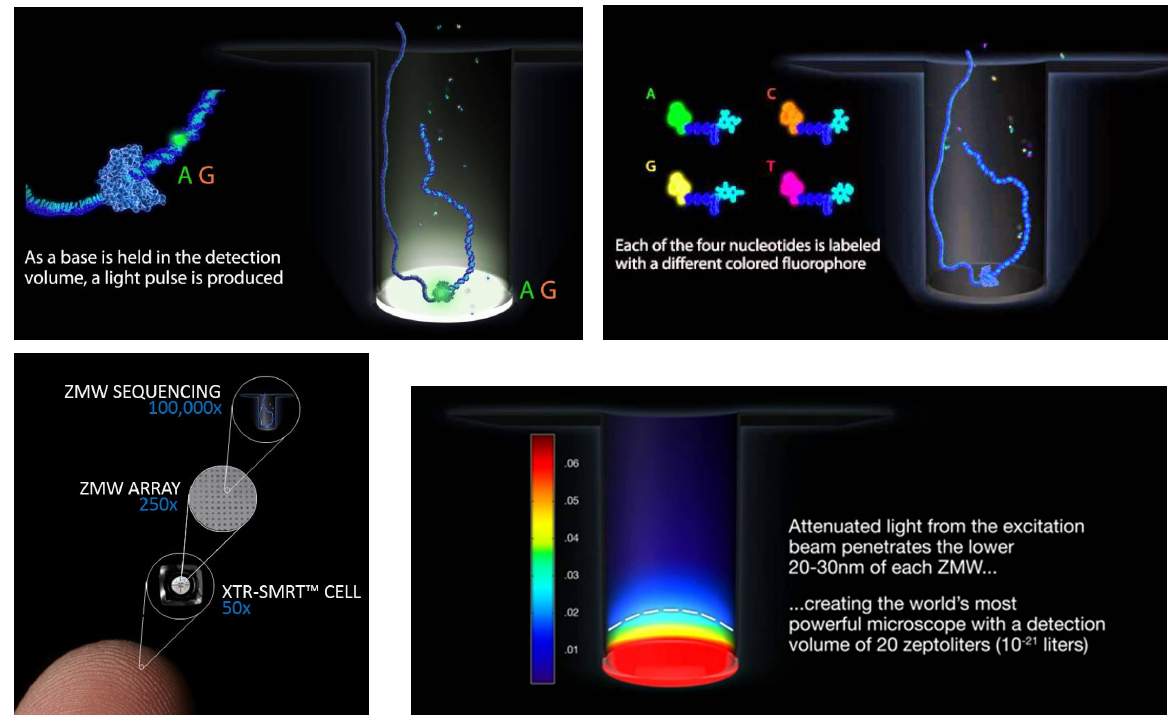
\includegraphics[width=1\textwidth]{PacBIO}
\label{}
\end{figure}


\subsection{Nanopore sequencing}
Intramembrane proteins are used, sequence detected through the passage of DNA nucleotides, which produce different voltage changes. During the first periods, this type of instruments gave great amount of errors, nowadays the technique is improving.
\href{https://www.youtube.com/watch?v=E9-Rm5AoZGw}{Nanopore Sequencing}

\graphicspath{{chapters/images/04/}}
\chapter{Sequencing data}
After all, genetics/genomics studies a code of a digital information (4bases/2bits). We should try to be as hypothesis driven as possible and use the already available and processed data to guide new data analysis. Be aware that, in genomics, data generation is the starting point of the study (the ratio of wet experiments vs computational effort is ~1:10)!\\
Given the biological problem at hand, we need to choose the optimal sequencing machine. To achieve this, we need to consider:
\begin{itemize}
\item Throughput;
\item Cost;
\item Read lenghts, 
\item Data output (reads per run);
\item Coverage; 
\item Seuencing errors (indel, substitution, CG delation, AT bias). Altough the error rate is decreasing wit new technologies;
\item Library preparation compatibility;
\item Speed (run time)
\end{itemize}
Suppose that we want to sequence a genome of a bacterium: which is the best machine that we can use?

\begin{description}
\item[Illumina NovaSeq]: if one wants to sequence a lot of DNA molecules at the same time, genomes, metagenomes. It can’t go over the 300 bp readlines runned, but it has the highest throughput so far (3TB of output). It is capable of multiplexing, so we have a unique barcode for any input sample. 
\item[Illumina iSeq]: If you need to sequence shorter genomes. From iSeq to NextSeq (increasing the reads lengths). 
\item[NanoPore (minion)]: pocket-sized wet-lab free sequencer for DNA, RNA and (possibly) proteins, but the read lengths is smaller than Illumina's. The machine is cheap; the running flow is more expensive (going down by time). It's a real-time sequencer. 
\item[PacBio]: carries a high amount of error. A solution to this is using more than one technology for the same project. For example, if the goal is to put together a genome of a bacterium, the challenge of using PacBio is errors in the sequence, while Illumina is unable to reconstruct the sample because there are ambiguities. By using both technologies, PacBio will construct the genome and Illumina will correct the sequence.\\
Anyway in the case of bacteria, you can use only PacBio because you have to sequence more and more, and since the PacBio error is random (not systematic), you will able to overlap the reads and solve the errors. PacBio has problem with homopolymers (same base or same set of bases repeated multiple times), which is a systematic error, more difficult to overcome just by sequencing more. If one wants to sequence a complex sample - with more than one genome - we cannot do the trick of overlapping, because we don’t know a priori which reads are coming from which organism. Another trick to work on this problem (complex samples), adopted by miniON and also PacBio, is to sequence the same molecule multiple times. By doing this you will have a molecule sequenced multiple times, and then we can go on with the other reads, and in conclusion do the consensus on that (sequencing error is usually declared by the machine). 

\section{Intro to sequencing raw data}

All sequencing platforms can produce FASTQ output files or they can at least convert their format to FASTQ. FASTQ contains the sequencing reads and the quality of each base and needs to be stored in a compressed format.\\
The first output is an internal output, not directly accessible by the user. You will see only the translation of the raw signal (FASTQ format). The internal raw signal can be completely different (ionTorrent measures pH, Illumina tkes photos of light signals, nanoPore looks at a signal coming from a little hole, …). However, all machines, internally, interpret this physical signal into a file which is in FASTQ format (the standard format). 
\\
Sequencing might lead to short (~100nt) strings of few digital values (A T G C), puzzles of ~3,000 M letters (solved then by assembling and mapping) or thousands of puzzles of ~5 M up to ~5,000 M letters, meaning ~3 TB of letters that need to be made sense of. Furthermore, many pieces do not fit due to sequencing error/SNP/structural variant or low complexity region/microsatellite/repeat.
\\
More on the FASTQ format will be covered in section \ref{subsection:fastq}.
\subsection{Base caller}
A base caller is an instrument (algorithm) inside the machine needed to understand how to work with the sequence, in particular, it translates the analogical signal of the reading into numbers/nucleotides. The most popular algorithm is \textbf{Phred}.
\\
Phred is an algorithm based on ideas about what might go wrong in a sequencing reaction and in electrophoresis. It was tested on a huge dataset of ‘gold standard’ sequences (finished human and C. elegans sequences generated by highly-redundant sequencing). Its results were compared with the ABI base caller and Phred was considerably more accurate (40-50\% fewer error). \\
NB: When things are getting too messy, the algorithm needs to understand that it is impossible to recover an high quality sequencing and so the base caller just needs to be able to give up for some reads (the ones without a high quality). The confidence that the base caller has to call a certain nucleotide ATCG is annotated in the FASTQ file, so one can later decide what to do with the bases that are not supported or clear.

\subsubsection{Errors solved by Ilumina's base caller}
\begin{description}
\item[Phasing noise $\phi$]: when a certain base is not seen frequently, the first time in which you will see this specific base (or pair of bases) there will be a peak (a spike) in the graph, increasing the signal of the nearby bases. There are going to be some errors in estimating the real nucleotide that is occurring in the site. This problem can be solved by waiting more time between a reading and another, but the sequencing will be less efficient (slower) and the throughput will be lower. So the machine needs to find a trade-off between the efficiency and the clear reading.
\item[Signal decay $\delta$]: after a while one has read the same base, or the same repeated couple of bases, the signal will go down and at some point will be indistinct (so at some point you will need to cut the read since it will be not trustable after a while).
\item[Mixed cluster $\mu$]: when you have a cluster mixed in two sequences, the machine will read the signal resulting by this two strings simultaneously. 
\item[Boundary effects $\omega$]:  in this case the machine needs to interpret an image (a digital object.. and a blue point will appear if you magnify it a little bit). To estimate the intensity of the blue charter here you should probably look at the internal part here and average out all the pixels. Putting the edge of the internal part is tricky, since it is a gradient and not clear.  So this error occurs when you can’t figure out what is the signal and what is the around background. 
\item[Cross-talk $\mathcal{X}$] %non nelle slides
\item[Fluophore accumulation $\tau$]
\end{description}

\subsubsection{Density on the flow cell}
There is an optimal clustering in the flow cell and the presence of readings that go one through the other represent a problem. In the case of the dark yellow spots, the one that are too closer are going to be considered as a single peak. It is even more a problem if the spots are of different colours, and the signal will be a result of different bases. 
\\
In the case of under clustered the machine doesn’t read simultaneously as many reads as it should do (and it is not a problem of the sequencing technology, it is a problem for the researcher who did not optimize the method). By increasing the flow’ density you will have an optimal clustering. If you increase the density too much you will have and over clustered sequencing. 

\subsubsection{An ecology of base callers}
With base callers the matter is finding a satisfying trade-off between accuracy and computational efficiency.
\\
The quality associated to a single nucleotide is internally estimated by the machine. We need to check later if the quality of the read is right. This quality is the estimation of the probability that that nucleotide in that position is wrong. 
\\
There's a difference between PHRED score reported by base caller vs. PHRED score when mapped to a reference sequence. There are some base callers more calibrated than the others (like the Ibis). In general base callers need to be calibrated with a standard to make sure that the estimations of the quality are accurate enough. 

\subsection{FASTQ format}
\label{subsection:fastq}

\begin{enumerate}
\item @SEQ\_ID 
\item GATTTGGGGTTCAAAGCAGTATCGATCAAATAGTAAATCCATTTGTTCAACTCACAGTTT x N 3. 
\item + 
\item !''*((((***+))\%\%\%++)(\%\%\%\%).1***-+*''))**55CCF>>>>>>CCCCCCC65 
\end{enumerate}

\begin{enumerate}
\item ‘@’ followed by a sequence identifier. The sequence identifier contains the unique instrument name, the flowcell and tile number, the x and y coordinates of the cluster within the tile, the index number for multiplexing and the pair number of paired-end sequencing. In Illumina MiSeq, each flowcell has 8 microfluidic channels (lanes), each lane contains three columns with 96 tiles, i.e. 96 multiplexed samples.
\item The sequence. It could be mate paired for paired end sequencing.
\item ‘+’, optionally followed by a sequence Identifier.
\item The quality scores. Quality is a number based on the estimated probability of error. $p$=probability  of error, $Q = -10 \dot p$ . We need a base quality of at least 20 to reach a small probability (1\%) [bq=40, p=0.01\%]. The FASTQ quality score is the phred score +33, converted in CHAR code.
\end{enumerate}
The FASTA file format is a FASTQ fomrat without the quality score reported and the seq ID is preceded by '>'.

\subsubsection{Quality control: read length distribution}
Quality scores are used typically for the operations of quality control and/or quality cleaning of the reads, which are then saved in FASTA files and used for other operations. However, since there exist algorithms, e.g. mappers, that take the reads and map them against a reference genome that can take into account the quality into a FASTQ directly. 
\\
Looking at the qualities will allow you to judge how well the sequencing run went. 
In this case, for example, the read length is used as quality control. In the second graph we can see that something went wrong, there are too many short reads. In this case you can use the sequencing results, but make sure to get rid of short reads when you do another sequencing, to have an optimal use of the machine. 
\\
Another way to look at your sequencing output is to look at the quality score directly. Here the quality goes down as the length of the reads increases. This is typical, since the machines have more and more problems in estimating the nucleotides when in continuum. In this case you can only cut the last results since the quality is too low. 
\\
Another problem that can occur is the adapter content. Sometimes it happens that you see the adapter, which should not be part of the sequencing reads, since the machine should be able to identify and remove it. This happens frequently when you have very short fragments in your output. After the machine has sequenced the sample, it starts to sequence also the adapter (if you don’t identify the end of the sequencing you will have the adapter in the sequencing output). The main solution is to remove the adapter and what follows it (but be aware that you will remove even the part of the sequence in the middle). 
\\
We can use FastQC to plot the quality distribution of our data. FastQC on 
Nanopore data: the reads are really long, but the quality is low (expected result). On PacBio data we also see the distribution falling entirely in the red zone, but here we have the box plot in the central part. 
\\
We can also plot differently the PacBio data. Here we still have PacBio, but in a different view. Instead of looking at each position separately, here we look at the average quality for the whole read. Probably you will discard the low-quality reads, like 1-2 score. When thinking at what technology use, think also at the length of the genome you want to sequence!

\subsubsection{FastQC on PacBio vs ONT}
The analyses were performed using long-read and short-read data from E. coli strain K12 sub-strains DH5$\alpha$ and MG16. Substitutions were more frequent in  ONT, while insertions were more frequent in PacBio. On nanopore A>G, T>C, C>T and G>A are 3 times more frequent than the other, while in PacBio the frequencies are more alike.
\\
\textbf{k-mer frequencies}: we know the frequency in the reference, so we assume that if the sequencing is systematic, without biases and without errors we should have the same frequency. In this example, it’s clear that nanopore has done a better job.
\\
(By looking at 6-mer you have a larger potential combination, but it is easier to find errors in it). Moreover, one can look at which are the over-represented and the under-represented k-mers in the reads compared to the genome, and this may give you an idea about where the errors are. Both in nanopore and PacBio, the most troubling k-mers are those containing the same repeated nucleotide (this is a frequent sequencing error).
\\
This is interesting because the low entropy of the repeated sequences can be detected by the quality control software and are usually discarded. We will see that sometimes it is not the right thing to do, since in non bacterial genomes there are repeated sequences (consideration to take when you decide which technology use for your experiment).

\subsection{Duplication artifacts}
It is not frequent to see duplication, but it can be a problem. If you want to reconstruct a genome from a scratch of a bacterium you don’t really care whether if there are duplicates or not. But if you want to quantify the gene expression or the copy number of genes in a bacterial genome, this can really skew your analysis. The distribution of the duplicates should be very similar to the distribution of the reads.
\\
There shouldn’t be any bias along the length of the reads.  If you see something like this, you probably sequenced the same thing over and over again, and so something went wrong. This happens when you sequence the adapter or the primer (they are always the same sequence).  

\subsubsection{GC content analysis}
We know that each single organism has a signature GC content. We expect to see a peak and a normal (gaussian) distribution. Therefor, if two peaks are seen, it means that we have sequenced two different organisms (maybe, a contamination). The problem is that these two organisms may share some sequences. 

\subsubsection{K-mers frequency plot}
Frequent k-mers can be a signature, as the GC content. For example: 15-mer coverage model fit to 76x coverage of 36bp reads from E. coli. 
The expected coverage of a k-mer with reads of length L:
\begin{equation}
L_{cov} = \frac{L-k+1}{L} \, \times \, Cov
\end{equation}
Than, given a k-mer, we can see in how many reads that k-mer was present. And in this case the coverage is around 40\%. However, there is a huge amount of k-mers present with coverage 1 (i.e. that you have seen only once in your reads). So, there are errors in that specific k-mers (remove these results). Instead, coverage higher than 80\% would mean that the k-mers are located in more than one position.

\subsubsection{Low-complexity artifacts}
Same nucleotide repeats (especially A) are in a lot of cases artifacts. It’s an error of the machine and the quality control looking at the quality scores, that in this case are very high.\\
How to measure their ‘artificiality’? Some parameters to take into consideration are:
\begin{itemize}
\item Low complexity 
\item Low entropy 
\item High compression (the artifacts increase the information inside the file) 
\end{itemize}
But some low-complexity sequences are not artifacts!
\begin{itemize}
\item Hydrophobic transmembrane alpha-helical sequences in membrane proteins 
\item CAG repeats in genes causing Huntington disease, spinal and bulbar muscular atrophy, dentatorubropallidoluysian atrophy. 
\item Proline-rich regions in proteins 
\item Poly-A tails in nucleotide sequence 
\item Micro-satellites 
\end{itemize}

\subsection{FASTQ quality control (QC)}
This is the first step (or sub-pipeline) in any NGS pipeline 
\begin{description}
\item[Clipping/trimming]: removing (low quality) parts of reads
\item[Masking]: avoiding to consider (e.g. low entropy) parts of reads
\item[Read removal]: discard low quality reads or reads that are too short after clipping
\end{description}

Additional features that can be exploited for QC are the GC content, clustering for contamination detection, TAG identification,ambiguous bases. 











































\end{description}
\chapter{Mapping}

Mapping (or aligning) and assembly are the operations that allow us to make some sense out of fragments (input data) deriving from sequencing, produce assemblies. 

\begin{itemize}
    \item \textbf{Mapping} is a key step in a modern genomic analysis and consists in the process of aligning the reads on a reference genome, in order to assign them to a specific location. With mapping, insights like the expression level of genes can be gained.
    \item \textbf{Assembly} by contrast, is the process of aligning and merging overlapping sequences in longer consensus sequences in order to reconstruct the original sequence/genome.
\end{itemize}

A consensus sequence is  the calculated order of most frequent residues, either nucleotide or amino acid, found at each position in a sequence alignment
In many cases, someone may have already assembled the genome or part of the genome (available reference sequences), so we don't need to do sequence assembly, only mapping (like for the human genome). Assembly will be needed however when studying new organisms. 

Problems related to mapping and assembly: 

\begin{itemize}
    \item absence of DNA fragments covering the gaps, makes it difficult to order the contigs (since there is no connection)
    \item presence of DNA artefacts (those must be discriminated with Quality Control)
    \item repeated sequences
\end{itemize}

\section{Mapping}

The coverage, or read depth, is the average number of reads representing a given nucleotide in the reconstructed sequence (Some points of the reference sequence will be aligned with more reads, some with less. The average number of reads for each nucleotide is the coverage). 
The coverage of a genome is defined as the average coverage of each single nucleotide across all nucleotides of the genome. Additional info and examples at:  
% https://thesequencingcenter.com/knowledge-base/coverage/#:~:text=Coverage%20is%20defined%20as%20the,reference%20genome%20Escherichia%20coli%20BW2952.
A coverage of 1x does not mean that all reads are read once. This would be true if sampling were systematic, but sampling is not systematic, it is random and is biased. Hence, a coverage of 1x means that on average each nucleotide is covered once, but there will be some nucleotides covered more and some not covered (0 coverage). 
The coverage can be represented with a coverage map and can also be defined theoretically as:
Cov = (N * L)/G
where G is the length of the genome; N is the  number of reads; L is the average read length.
Knowing the wanted coverage is important to set up the machine in order to obtain the right number of reads (to achieve a certain coverage). A higher coverage means indeed more reads to be obtained. 

\subsubsection{Exercise on coverage}

\emph{How many reads do I need to cover the entire genome?}
Define the probability  to cover the full genome (with a certain epsilon subtracted - so not 100$\%$) or: define the number of reads N to cover the whole genome with a certain probability P = 1- epsilon.

\begin{figure}[h]
\centering
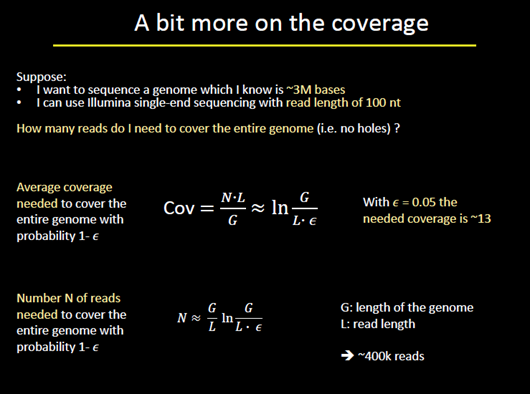
\includegraphics[width=0.6\textwidth]{coverage.png}
\caption{}
\end{figure}

In general, the sequence mapping process consists in performing comparisons between experimental sequence data (reads obtained with sequencing) with some reference information, like reference genomes and known genes (eg. the human genome). The comparison can lead to obtaining new information, such as the presence of SNPs which can be linked to pathological conditions or whatsoever, based on the starting point.

\begin{figure}[h]
\centering
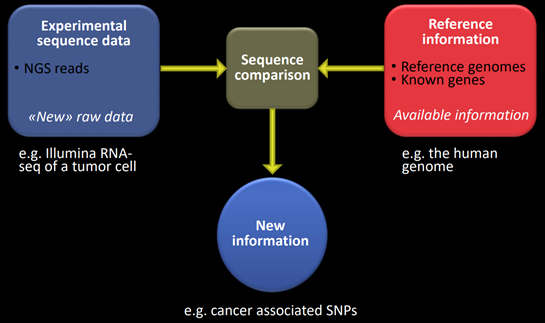
\includegraphics[width=0.6\textwidth]{SequenceComparison.png}
\caption{}
\end{figure}

\section{Mapping algorithm}

Over time many different mapping algorithms were implemented; some of them are not used anymore, while others are the base of current mapping and aligning genomic tools. 
Ideally, the \textbf{simplest aligning algorithm} could consists in:  
We have a smaller sequence that we want to align to a longer one. Start from the first position, align the query sequence against the subject, and look at how many nucleotides are correct (score: 4/10 = 40$\%$), then repeat for all positions until a perfect match is found (if found). The problem with this algorithm is that it doesn't consider insertions and deletions.

\subsection{Local vs Global alignment}
Sequence alignment can follow two different approaches.

\begin{enumerate}
    \item In \textbf{global alignment} an attempt is made to align completely the 2 sequences (end to end alignment). So global alignment finds the best alignment across the whole two sequences. This approach is suitable for comparing closely related sequences like homologous genes. 
    \item \textbf{Local alignment}, on the other hand, focuses on finding regions of similarity in parts of the sequences (so it aligns subsequences of the query sequence to a subsequence of the target sequence). This approach is suitable for aligning more divergent sequences or distantly related sequences. Used for example for finding out conserved patterns in DNA sequences of motifs in two proteins.
\end{enumerate}

Sequence similarity is connected with \textbf{evolutionary distance} (also for cell populations in a tumour). Very high similarity implies a very low distance. But when the similarity goes down and reaches the twilight zone, it is more difficult to define the evolutionary distance and to give meaning to results (the zone depends on the experiments).

\begin{figure}[h]
\centering
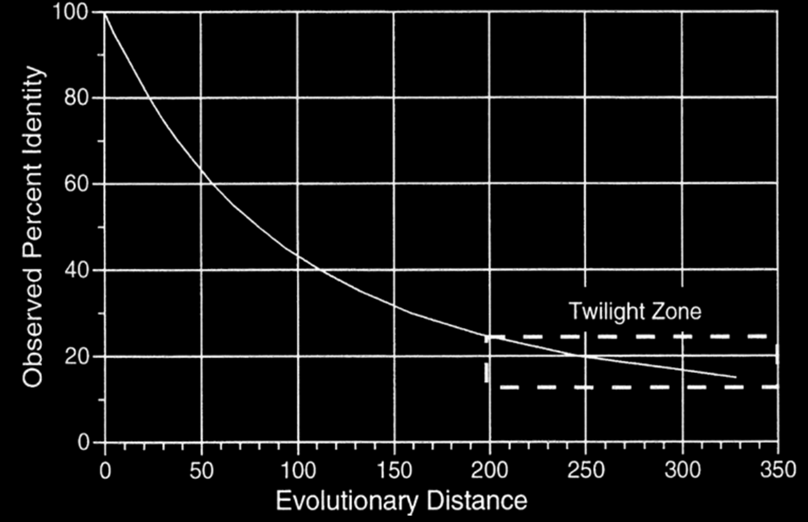
\includegraphics[width=0.6\textwidth]{EvolutionaryDistance.png}
\caption{}
\end{figure}

\subsection{Smith-Waterman algorithm  (local alignment) - 1981}

%Paper link: https://www.sciencedirect.com/science/article/abs/pii/0022283681900875?via%3Dihub
Take the algorithm for string recognition and apply it to find common molecular sequences. Not good for indels and substitutions. 
The S-W Algorithm is a local-alignment algorithm based on dynamic programming, whose aim is to find the best match among all possible (optimal local alignment) with respect to the scoring system used .
Firstly, we need to define a \textbf{score} for matches and penalties for mismatches and gaps (defined by the formula). 
The algorithm starts by putting zeros in the first row/column (\textbf{INITIALIZATION}). Then, starting from the first position H(1,1), at each iteration a number, based on the formula, is added (\textbf{ITERATION}). The number to be added is the greater between the 4 numbers defined by the formula, where d represents the penalty for gaps, and  s(x,y) = score when 2 NTs are the same (This gives a score of 5 if the 2 bases are equal, -3 if they are different) (PARAMETER SETTING).

\begin{figure}[h]
\centering
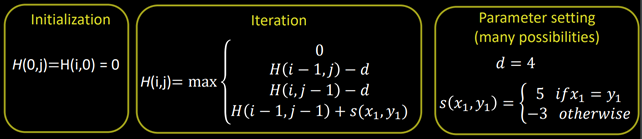
\includegraphics[width=0.6\textwidth]{Waterman.png}
\caption{}
\end{figure}

\textbf{Example}

First position H(1,1) = (G,C), max between: 

\begin{itemize}
    \item 0
    \item H(i-1, j) = 0-4 = -4
    \item H(i, j-1) = 0-4 = -4
    \item H(diag) + s(x, y) = 0 – 3 = -3
    \item $\xrightarrow[]{}$ We put 0
\end{itemize}

Second position H(2,1) = (A, G):

\begin{itemize}
    \item - 0
    \item -4
    \item -4
    \item -3
    \item $\xrightarrow[]{}$ We put 0
\end{itemize}

Third position H(3,1) = (C e C):

\begin{itemize}
    \item - 0
    \item -4
    \item -4
    \item 0 + 5 (since C=C)
    \item $\xrightarrow[]{}$ We put 5 
\end{itemize}

Here we also put an arrow indicating the nucleotide in the diagonal, to indicate that the 5 score derived from that point (hence from that path).  The arrows are needed to reconstruct the alignment at the end of the process. The iteration is performed for each cell of the table (column wise).
The parameters chosen for d (gap penalty) and s(x,y) (match or mismatch) can change the results. 
Final Solution: 

\begin{figure}[h]
\centering
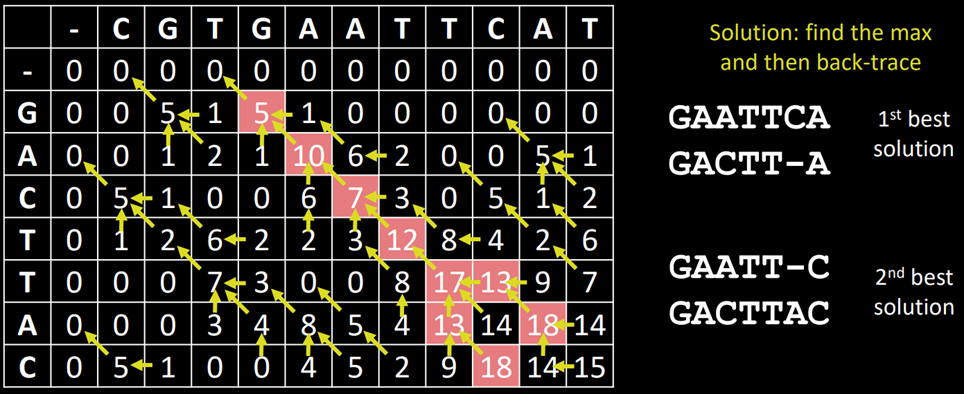
\includegraphics[width=0.6\textwidth]{Aligning.png}
\caption{Aligning CGTGAATTCAT and GACTTAC}
\end{figure}

Find the \textbf{maximum number} (18, here we have 2 of them) and go back following the arrows. In case of multiple highest scores, traceback should be done starting with each highest score.
From this path, the sequence is constructed by these rules:

\begin{itemize}
    \item A diagonal arrow represents a match or mismatch, so the letter of the column and the letter of the row of the origin cell will align.
    \item A horizontal or vertical arrow represents an indel. Vertical arrows will align a gap ("-") to the letter of the row (the "side" sequence), horizontal arrows will align a gap to the letter of the column (the "top" sequence).
    \item If there are multiple arrows to choose from, they represent a branching of the alignments. If two or more branches all belong to paths from the bottom right to the top left cell, they are equally viable alignments. In this case, note the paths as separate alignment candidates.
\end{itemize}

This algorithm is not used anymore due to a too high computational expense (huge number of comparisons for real genomes) and storage (memory and speed). In fact comparing two Eukaryotic genomes will result in a excessively great aligning matrix ($\sim$3Gb x $\sim$3Gb), and also using small reads against the human genome is unfeasible: 100 x $\sim$3Gb for each read!

\subsection{Needleman-Wunsch algorithm (global alignment)}

This global alignment algorithm was developed in 1970 and is also based on dynamic programming. The purpose of the algorithm is to find all possible alignments having the highest score. Again, a scoring system must be defined, then the algorithm proceeds in a similar way as the SW. 

\begin{figure}[h]
\centering
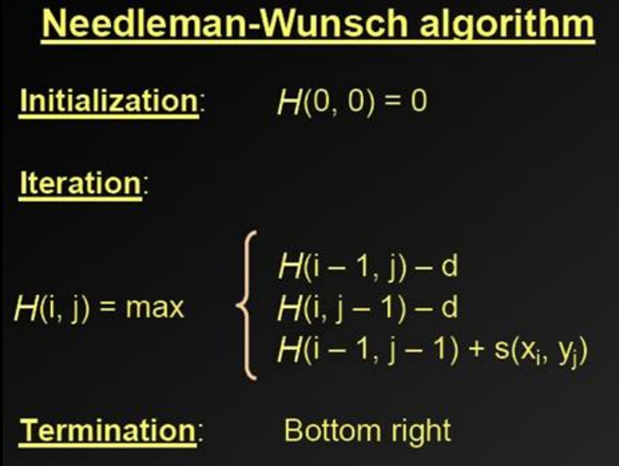
\includegraphics[width=0.6\textwidth]{Needleman.png}
\caption{}
\end{figure}

The differences are:

\begin{itemize}
    \item Initialization: we start from only one value, one zero, putted in H(0,0) (need to start from the first nucleotide - global). 
    \item The formula contains no 0 anymore, it adds the maximum score between 3 possible scores, we are always comparing with the first nucleotide of the sequence. 
\end{itemize}

\begin{figure}[h]
\centering
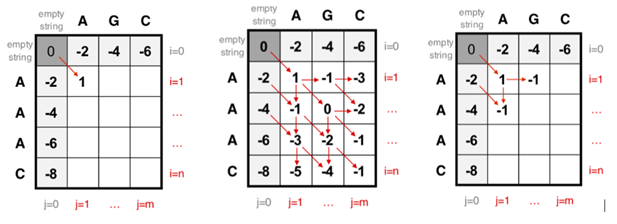
\includegraphics[width=0.6\textwidth]{Needleman2.png}
\caption{}
\end{figure}

New algorithms were implemented later. 
BWA and BowTie2 are the best ones available right now for short reads. Blast could go too but it would take a lot of time. 

\begin{figure}[h]
\centering
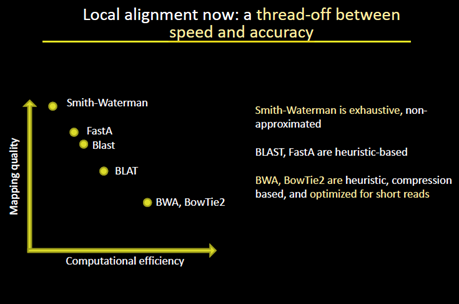
\includegraphics[width=0.6\textwidth]{LocalAlignment.png}
\caption{}
\end{figure}

The methods going from FastA to BowTie2 are \textbf{heuristic methods}: the solution found does not need to be the best one, but the best approximation given certain parameters (like time). Also, Blast gives an answer based on a fixed level of sequence similarity (in a reasonable amount of time) and gives no result under that level. So Blast online is not very sensitive, it is trained to provide only very good results to not overload the servers. 
A \textbf{heuristic}, or heuristic technique, is any approach to problem solving or self-discovery that employs a practical method that is not guaranteed to be optimal, perfect, or rational, but is nevertheless sufficient for reaching an immediate, short-term goal or approximation. Where finding an optimal solution is impossible or impractical, heuristic methods can be used to speed up the process of finding a satisfactory solution. Heuristics can be mental shortcuts that ease the cognitive load of making a decision.
BWA and BowTie2 are also ‘compression based’ algorithms, meaning that they exploit data compression techniques in order to compress reference genome files to reduce the number of bits used to encode the document (better explained below).

\subsection{BLAST (Basic Local Alignment Search Tool)}

%Tutorial: https://www.youtube.com/watch?v=HXEpBnUbAMo&ab_channel=JHUAdvancedAcademicPrograms
Despite its limitations, Blast is still used a lot and when it was first released it revolutionised the field making sequence alignment available for anyone and for any computer (it can be run online).
How does it work? Steps:

\begin{enumerate}
    \item \textbf{Seeding}: find perfect or almost exact k-mer matches (series of sequences with defined length). The idea is to look for identical short matches and try to expand from that. 
    \item \textbf{Extension}: extend the seeds at point one 1 with possibly some non-exact but high-score matches, that permit to obtain better alignments.
    \item \textbf{Evaluation}: create alignments for the regions of high-scoring extended seeds. Every time the statistical significance of the match is evaluated with methods inspired on the NW and SW approaches.  
\end{enumerate}

In online Blast tools the seed is set to 25/29. If a sequence of that length does not match perfectly another sequence we will have no results. One solution would be to lower the seed, but this cannot be done online because it would take too much time. Another option is to reduce the dataset in which we search.
There are many types of blast available, shown in figure:

\begin{figure}[h]
\centering
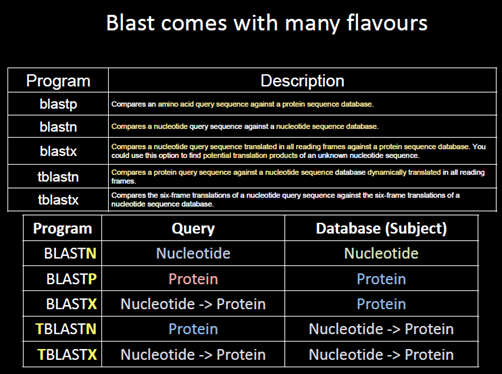
\includegraphics[width=0.6\textwidth]{Blast.png}
\caption{}
\end{figure}

\textbf{Scoring matrices} are very important especially for amino acids, they are used to score alignments between protein sequences. Blosum 62 (BLOcks SUbstitution Matrix) is one of the most used.
They put non simple penalties in substitutions of different amino acids, for example based on the functional properties of the substitutions. A scoring matrix contains values proportional to the probability that amino acid i mutates into amino acid j for all pairs of amino acids. Such matrices are constructed by assembling a large and diverse sample of verified pairwise alignments of protein sequences.
Other \textbf{parameters} can be set in online BLAST:

\begin{itemize}
    \item Max target sequences $\xrightarrow[]{}$ number of reported sequences 
    \item Expected threshold $\xrightarrow[]{}$ e-value
    \item Words size $\xrightarrow[]{}$ seed
    \item Gap cost $\xrightarrow[]{}$ cost for adding multiple gaps. Linear = twice the gap penalty (if I have to add a second gap after another one).
    \item Filter low complexity regions to avoid getting stuck 
\end{itemize}

\subsubsection{BLAST E-value}

If we have a match and the database is random, how many other matches I will likely find?

\begin{figure}[h]
\centering
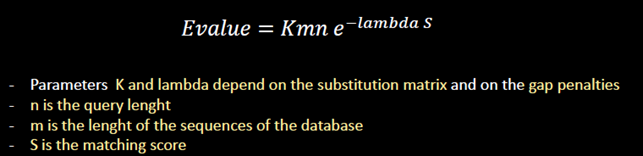
\includegraphics[width=0.6\textwidth]{Evalue.png}
\caption{}
\end{figure}

The \emph{e-value} represents the number of distinct alignments with a score equivalent to or higher than S, that are expected to occur in a database search by chance. An e-value of 10 means that up to 10 alignmentscan be expected to be found just by chance, given the same size of a random database. E-value can be used as a first quality filter for the BLAST search result, to obtain only results equal to or better than the number given by the e-value option. Blast results are sorted by E-value by default (best hit in first line).
The smaller the e-value, the better is the match. A small e-value means a low number of hits, but of high quality, whereas a high e-value indicates many hits, partly of low quality (if the number of better possible alignments is high, it means that it is particularly probable to find by chance an alignment which is better the the one found, and so it is more probable that those alignments are bad). 
There is a relationship between the E-value and the p-value. 

\begin{itemize}
    \item The E-value is the number of sequences that we would find by chance;
    \item The p-value measures the probability of finding by chance another sequence with an equal or better score.
\end{itemize}

%aggiungi formula

\subsection{Speed seed alignment}

There are algorithms implemented 10/15 years ago that focus on seeds -> not used anymore. 
Those methods cut both the reads and the reference sequence (read-sized pieces of reference sequence) into small seeds. The reference seeds are then stored in an index (hash look-up table).
The idea is to do that for all possible k-mers. Eg. we choose a seed of 10: the first starts at position 1, the second at position 2, ecc. And then to look up seeds for each read and identify the positions in genome where spaced seed pair is found. 

\begin{itemize}
    \item 1 SNPs means that at most 1 seed is not-matching
    \item X SNPs means that at most X seeds are not-matching
\end{itemize}

Algorithms based on this approach are: Maq, SOAP, MOSAIK. 
Problem: the lookup table (the reference) for the human genome is too big: 50Gb $\xrightarrow[]{}$ problem in RAM.

\subsection{Burrow-Wheeler alignment}
This algorithm is based on a very efficient way to store the reference genome, based on the BW transformation, that allows to have a reference index which is way lighter (with respect to the spaced seed approach); in fact, at the end of the transformations, equal letters are next to each other. It is successful because the database is compressed and does not need to be decompressed. However, when we compress a file, the compression must be reversible. There must be a way to go from the BW compressed/transformed index to the original one, to find reads in the genome. 
The search is based on finding suffixes of the reads in the BW structure. With this approach the index of the human genome is around 2GB. The algorithms BW-based are the fastest currently available. 
BWT is also used in text compression.
Example:
We want to compress the word BANANA
\begin{itemize}
    \item - we take all the rotations of the word
    \item we sort them based on lexigographic order (Lex order - lexicographical order is a generalization of the alphabetical order of the dictionaries to sequences of ordered symbols) 
    \item we take the last column
\end{itemize}

We end up with a string which is more compressible, there are sequences of the same letters that can be described at a higher level (Eg. there is 1 B, 2 NN, ecc)
In the method shown, in order to \textbf{reverse the transformation} and go back to the original word, the input sequence (output of the compression) is added as a column and then sorted (based in lex order), and this two passages are repeated as many times as are the characters of the sequence (8 in this case), obtaining at the end a matrix with equal number of columns and rows. As a result we go back to the ordered sequence of the word's rotations, in which the last one (last line) is the original input string. 
It takes a lot of time but it makes it reversible; plus, there are actually smarter ways to go back, such as ones base on the LF property.

\subsection{LF (Last-First) property}

As in the previous method, the first step consists in sorting all word's rotations and taking the last column which will be the compressible one.
The LF property is then applied to the list of all rotations,
to get back to the input sequence, by following this principle: the ith occurrence of character X in the last column corresponds to the same text character as the ith occurrence of X in the last column.
Example: We want to reverse the transformation of the string "gc$\$$aaac”. 

\begin{figure}[h]
\centering
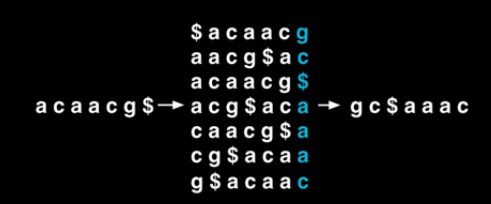
\includegraphics[width=0.6\textwidth]{1LF.png}
\caption{}
\end{figure}

\begin{figure}[h]
\centering
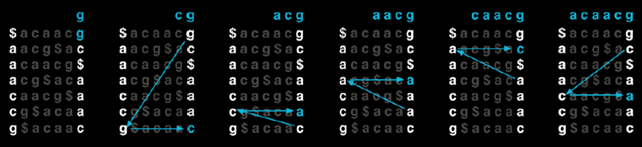
\includegraphics[width=0.6\textwidth]{2LF.png}
\caption{}
\end{figure}

\begin{itemize}
    \item \emph{g} is the first occurrence of g in the last column and corresponds to (arrow) the first occurrence of \emph{g} in the first column. Tracing a horizontal arrow gives the next nucleotide.
    \item \emph{c} is the second occurrence in the second column and corresponds to (arrow) the second occurrence of \emph{c} in the first column. Tracing an horizontal arrow gives the next nucleotide.
    \item \emph{a} is the third occurrence of a in the second column and corresponds (arrow) to the third occurrence of \emph{a} in the first column. Tracing an horizontal arrow gives the next nucleotide.
\end{itemize}

And so on. Each time we keep track of the character that we are looking at and we end up by constructing the original word. With this method we reconstruct the word from its end to its beginning (backward). 

\subsection{Exact mapping using LF property}

In mapping, we can look for sequence matches using the compressed database.
Backward exact mapping works by calculating the range of matrix rows beginning with successively longer suffixes of the query.
Example: we want to match the string 'aac' with the database.

\begin{figure}[h]
\centering
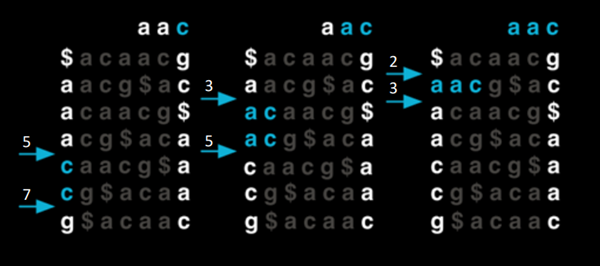
\includegraphics[width=0.6\textwidth]{3LF.png}
\caption{}
\end{figure}

\begin{itemize}
    \item we take the 'first suffix' \textbf{c} of the query string and we look for it in the first column. We find 2 matches in lines 5 and 6, so in the range 5-7.
    \item we pass to a 'second longer suffix' \textbf{ac} and see if we can find it in the matrix $\xrightarrow[]{}$ lines 3 and 4, range 3-5.
    \item we look at the suffix \textbf{aac} and find it in the 2-3 range.
\end{itemize}

Doing the backward matching we exploit the characteristics of the BWT transform. This same approach could be used to find a match between a query read and a reference genome which has been compressed using the BW alignment.
The problem is that it does not take into accounts indels, mismatches. 
A possible solution to this problem could be the \textbf{inexact mapping}. 
Perform exact mapping and, if the query is not found, go back and perform backtracking by hypothesising mismatches. For example we want to find a match for the query GGTA. As always, we start looking for a match starting from the last character.

\begin{itemize}
    \item we find a match for a, t, g but not for the last g. 
    \item so we go back and hypothesize a mismatch for the first letter a. We then look for all the matches that we could find if we replace a with another nucleotide (we do the same for the other NTs in the query?). 
    \item we find than by replacing a with a g, we find a match (ggtg) (not exact match).
\end{itemize}

The Burrows-Wheeler algorithm is used in BowTie and Bowtie2. 
Right now there are many algorithms to choose between and many review papers compare their characteristics and performance. No tool outperforms the others in all the test, hence the decision of which algorithm to choose must depends on the specific needs. 

\begin{figure}[h]
\centering
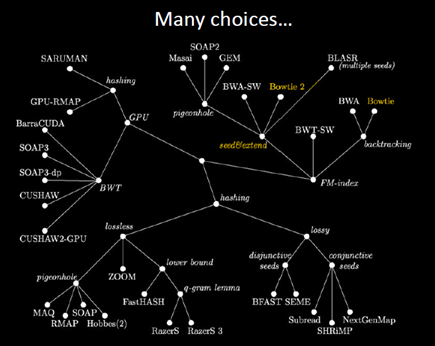
\includegraphics[width=0.6\textwidth]{Choices.png}
\caption{}
\end{figure}

\chapter{Assembly}

\graphicspath{{chapters/images/07}}
\chapter{16S-rRNA sequencing}

\section{Introduction to metagenomics}

  \subsection{Definition of metagenomics}
    The term \textbf{metagenomics} refers to the "\textit{study of \textbf{uncultured microorganisms} from the environment, which can include humans or other living hosts}" whith "\textit{focus on taxonomic and functional characteristics of the \textbf{total collection of microorganisms} within a community}". The main way to analyze the entire microbial population of an environment is through \textbf{high-throughput sequencing} of nucleic acids isolated from the sample; we can further distinguish two approaches, namely \textbf{16S rRNA gene sequencing} and \textbf{shotgun  metagenomics}.

  \subsection{Why studying the metagenome}
    Microbes are basically everywhere, in and outside of our bodies, in oceans, glaciers, hot springs and rocks. Given how widespread and abundant microbes are, studying the metagenome provides us plenty of information (both on human and non-human microbiome and environment). For instance, it has been shown that the microbiome correlates to several diseases, therefore it can be used as a non-invasive \textbf{biomarker} (colorectal cancer, immunotherapy efficacy, autoimmune diseases...); the list of activities microbes are involved in is evergrowing.

  \subsection{Differences with older microbiome studies}
    The microbiome was discovered many years ago but there were no tools to analyze it properly; the only way was to culture and isolate each bacterium, which is an unfeasible approach to study the entire community, since only some bacteria can be grown in lab and it still would take an unreasonably long amount of time. The advent of high-throughput technologies is what made possible to study the microbiome of a sample, reducing significantly times, costs and increasing substantially the fraction of the microbiome that can be known.

  \subsection{Example: skin microbiome}
    Some studies were performed on skin microbiome (Segata et al, Nature Methods 2012, Truong et al, Nature Methods, 2015); only about 60\% of the contigs (of various size) were mapped to known microbes while 40\% belonged to unknown species. When separating these sequences based on GC content and abundance, many clusters formed, some with higher abundance while others with lower abundance, probably due to the low GC content that makes more difficult for the machine to sequence them, therefore causing them to be underestimated. Studying this 40\% of unknown sequences is one of the main tasks of metagenomics.

\section{16S rRNA sequencing}

  16S rRNA sequencing is one of the first techniques developed to study the microbiome, since it does not require a huge amount of sequences nor excessive costs; for these reason the technique became popular.

  \subsection{Simplified 16S rRNA analysis workflow}
    The general workflow for a 16S rRNA analysis is the following:
    \begin{itemize}
      \item \textbf{DNA extraction} from the entire community present in the sample; some bacteria will be over-represented while other will be under-represented.
      \item \textbf{Selective PCR amplification of 16S rRNA gene} (due to the characteristics explained below)
      \item \textbf{High-throughput sequencing}
      \item \textbf{Sequence mapping} against genomes in databases; this allows to define which bacteria (and which variants of those) are present in the sample and to find new and unknown bacteria.
    \end{itemize}

    \begin{figure}[!h]
      \centering
      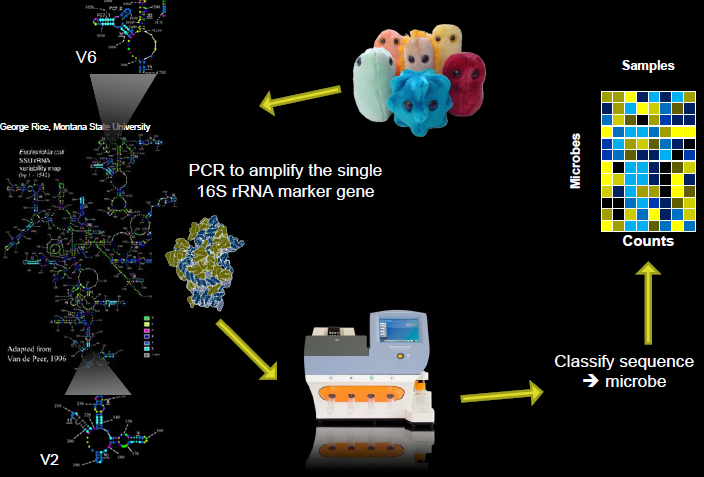
\includegraphics[width=0.9\textwidth]{general_workflow.png}
      \caption{\label{fig:general_workflow}General 16S gene analysis workflow}
    \end{figure}

  \subsection{16S rRNA gene}
    The ribosome is one of the most conserved, if not the most conserved, structure in all living organisms, making it one of the best phylogenetic markers. In prokaryotes, the ribosome is composed of several elements, both proteic and RNA based. Of the RNA based ones, 3 of them are \textbf{ribosomial RNAs} (rRNAs), namely 5S, 16S, 23S. Since these components are fundamental for any bacterium, all bacteria present the genes codifying for these rRNAs; most of the sequences are highly conserved but some regions have some variability which, since this variability is species-specific, can be used as a \textit{barcode} to find and classify species (it also allows to distinguish between Archea and Bacteria).
    The most conserved of the rRNAs is 23S but the one used for microbiome analysis is 16S (which corresponds to the human 18S). The 16S rRNA gene is a few thousands nucleotides long, most of which are highly conserved; the bulk of the differences among species is in the hypervariable regions (named V1 to V9), which are terminal loops of the structure (basically regions far away from the catalityc site, therefore more free to mutate). Despite the high degree of conservation, some variability can be found outside the hypervariable regions too (eg. 530 loop structure).
    The annotation of which portions of the 16S rRNA gene are conserved has been performed using \textit{E. coli} as a reference; for a few hundred organisms the gene has been compared to the reference one to define the degree of conservation of each stretch of nucleotides. Some totally conserved regions (meaning pretty much identical in all species) are present but they are not very big.

    \begin{figure}[!h]
      \centering
      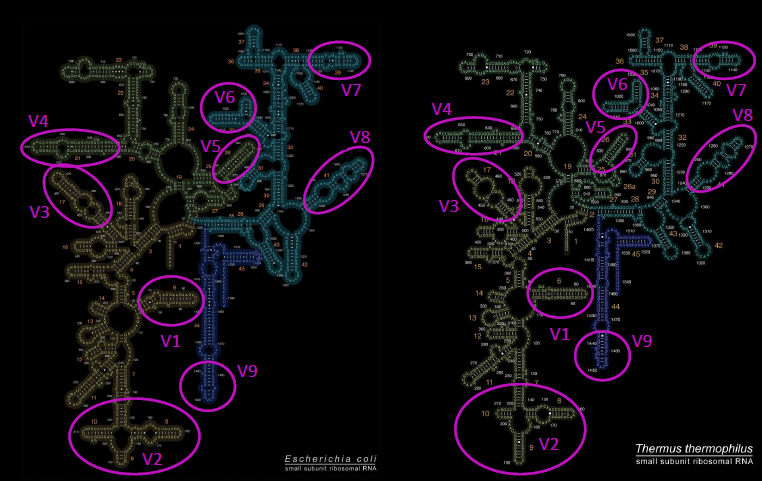
\includegraphics[width=0.9\textwidth]{16S_rRNA.png}
      \caption{\label{fig:16S_rRNA}Structure of the 16S rRNA in \textit{E. coli} and \textit{T. termophilus}}
    \end{figure}

  \subsection{Primer and high-throughput machine choice}
    One could sequence the entirety of the 16S rRNA gene, for example using NanoPore seq, but this would introduce many errors that could lead to mapping the sequence to the wrong organism; for this reason it is preferred to amplify only certain specific regions of the gene.
    To study the microbiome in a high-thoughput way you need primers which can bind to all species, but since the sequences conserved in all species are too short, you use primers that bind highly conserved regions; for this reason, regardless of which primers you choose there will be bias in your results (some species will not be identifiable using those primers). This bias can be somewhat minimized using \textit{in silico} primer validation, which means testing your primers against databases of 16S tRNA genes (silva and green genes), to test and decide the best pair of primers for your experiment.

    \begin{figure}[!h]
      \centering
      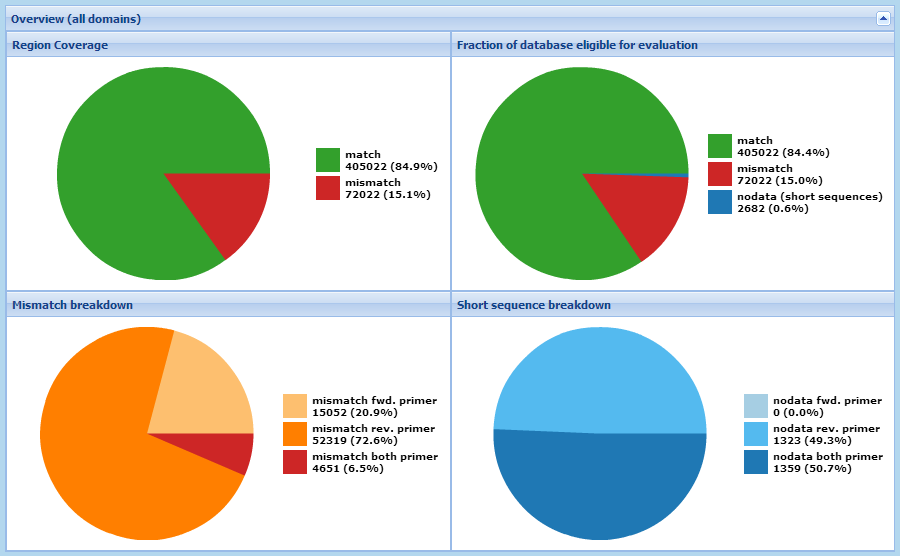
\includegraphics[width=0.9\textwidth]{silva_analysis.png}
      \caption{\label{fig:silva_analysis}Example of \textit{in silico} primer validation using silva; you can notice the different efficiency of the primers relative to different parameters.}
    \end{figure}

    Still, two experiments conducted with different primers will always have some differences.
    Moreover the binding regions must flank some variable region, in order to include it in the amplicon; finally you need pair end amplification (both primer back and forward) in order to have the complete amplicon (to make comparison easier). Given these characteristics there are multiple possible priming sites, based on the sequence and on chemical properties of the primers. Moreover, primers can be used as forward or reverse to obtain different combinations and sequences.

    \begin{figure}[!h]
      \centering
      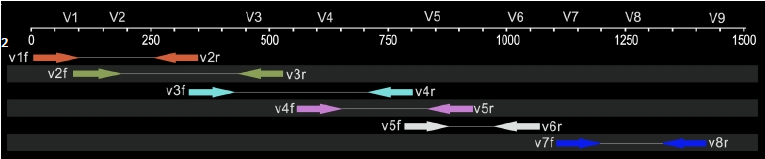
\includegraphics[width=0.9\textwidth]{primer_placement.png}
      \caption{\label{fig:primer_placement}Examples of common primer placements relative to hypervariable regions}
    \end{figure}

    As an example of the importance of the choice of primers, in some skin microbiome analyses, researchers could not find two bacteria always present on human skin due to the choice of primers. Moreover \textit{S. aureus} seemed over-represented due to the non-amplification of other important species. Despite the biases, this technique is still extremely useful even today.

    There are different protocols to target conserved regions also based on the machine used. In general:
    \begin{itemize}
      \item Sanger machines are not very good for this application since they have low throughput and they are more suited for longer sequencing tasks (full genomes for instance)
      \item Roche 454 machines have historically been well suited, since it was possible to sequence three hypervariable regions toghether using 400 nucleotides reads, providing a good cost/throughput trade-off.
      \item Illumina HiSeq is not the optimal choice since it has shorter reads and unnecessarely high througput; Illumina MiSeq and IonTorrent can be a decent compromise.
    \end{itemize}

  \subsection{In depth 16S rRNA analysis workflow}
    A more in depth 16S rRNA analysis worflow is the following:
    \begin{itemize}
      \item \textbf{DNA extraction} from each of your samples
      \item \textbf{Selective PCR amplification of 16S rRNA gene}, introducing a barcode in the sequences using tagged primers.
      \item \textbf{High-throughput sequencing} of all the samples in a single run (to reduce costs); the result is a set of amplicons belonging to different samples and with a barcode attached.
      \item \textbf{Demultiplexing}, which means removing the barcodes and assigning each sequence  to the corresponding sample. Sequencing noise must be taken into account, therefore low quality reads must be removed.
      \item \textbf{Multiple sequence alignment} against reference sequences. Some reads will probably not map to any reference sequence.
      \item \textbf{Group related sequences into OTUs} (operational taxonomic units), which means grouping sequences that share some common variants; since there are some SNPs in the microbial genome, the similarity threshold between sequences cannot be too restrictive. OTUs can be used to define the relative abundance of each species in the sample, but in order to do so it is necessary to normalize for the copy number of the 16S gene sequence; this is very difficult since an accurate estimate can be made only if long reach sequencing has been performed on the organism, which is almost never the case since for microbes that basically corresponds for full genome mapping (needless to say it is therefore non applicable on unknown microbes).
      \item \textbf{Build phylogenetic tree} using one representative for each OTU.
      \item \textbf{Annotate} the OTUs using 16S gene databases.
      \item \textbf{Downstream analysis} is performed, such as clustering to visualize similarities among samples.
    \end{itemize}

    \begin{figure}[!h]
      \centering
      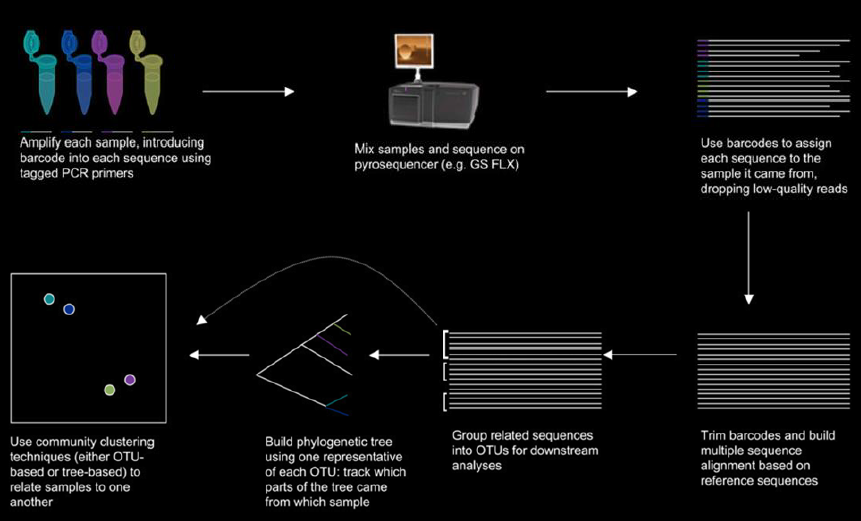
\includegraphics[width=0.9\textwidth]{expanded_workflow.png}
      \caption{\label{fig:expanded_workflow}Expanded 16S gene analysis workflow}
    \end{figure}

    \begin{figure}[!h]
      \centering
      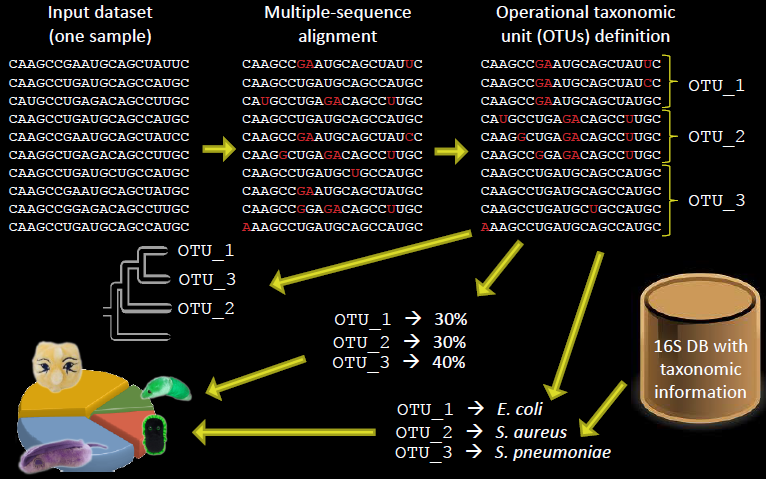
\includegraphics[width=0.9\textwidth]{zoom_in_16S.png}
      \caption{\label{fig:zoom_in_16S}Zoom in on 16S gene analysis workflow}
    \end{figure}

  \subsection{OTU clustering}
    Defining OTUs requires using multiple sequence alignment; since this approach is a generalization of the mapping algorithm (meaning you have to compare every sequence with every sequence) it is quite complex in terms of speed, but still feasible. Generally, greedy algorithms, which add the lowest possible amount of gaps, are used to perform multiple sequence alignment. After the alignment, sequences are split into OTUs (operational taxonomic units), which are basically groups of 16S sequences very similar to each other. Generally a sequence is defined as the representative of the OTU, meaning that it has a certain threshold of identity with all other sequences in the OTU (usually 97\% when considering species) and that minimizes the differences of all other sequences of the OTU with itself. Some OTUs can be assigned univocally to a species, some others may be associated to more species, some others cannot be mapped to know species. The fact that a species may map to multiple OTUs is often a negative factor (confusion in the analysis) but it may sometimes allow to find subspecies.
    \begin{figure}[!h]
      \centering
      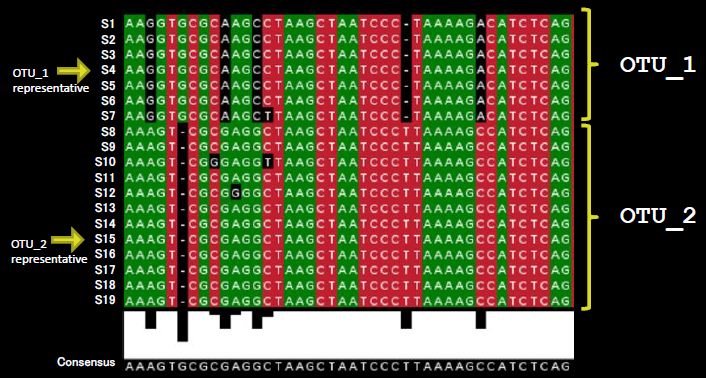
\includegraphics[width=0.9\textwidth]{OTU_general.png}
      \caption{\label{fig:OTU_general}Example of multiple sequence alignment for OTUs}
    \end{figure}

    After sequence alignment, OTU clustering (= splitting the sequences into OTUs), can be done through several supervised or unsupervised learning methods. Each methods has pros and cons, therefore there is not an always optimal method.
    The most common unsupervised clustering methods are:
    \begin{itemize}
      \item \textbf{Single linkage clustering} (nearest neighbour): assign the sequence to a cluster if that OTU already contains \textbf{at least a sequence} similar enough (97\%). However two distant sequences in the OTU network could share a similarity which is way lower than 97\% (because of a series of connections above 97\%); this could result in \textbf{underclustering} (defining too few clusters).
      \item \textbf{Complete linkage clustering} (furthest neighbour): assign the sequence to a cluster only if \textbf{all the sequences} of the OTU are similar enough (97\%). However two sequences may be similar enough (97\%), yet belong to different OTUs, because the overall cluster width, or \textbf{divergence}, is at most 3\%; this approach could then generate different solutions, based on the order the points are added in. Moreover, if the clustering conditions are too stringent, sequencing errors and SNPs in the microbial genome may result in \textbf{overclustering} (defining too many clusters).
    \end{itemize}

    \begin{figure}[!h]
      \centering
      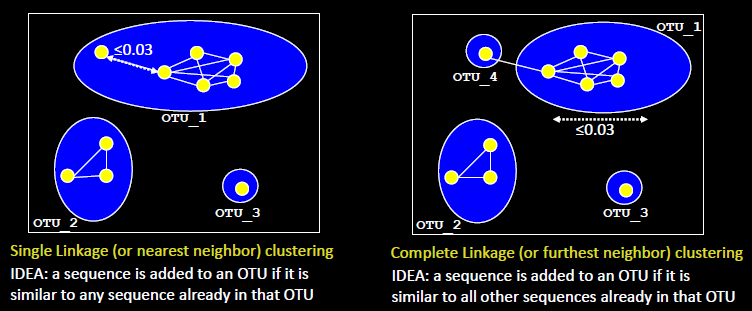
\includegraphics[width=0.9\textwidth]{clustering_methods.png}
      \caption{\label{fig:clustering_methods}Visualization of single linkage analysis and complete linkage analysis}
    \end{figure}

    \begin{figure}[!h]
      \centering
      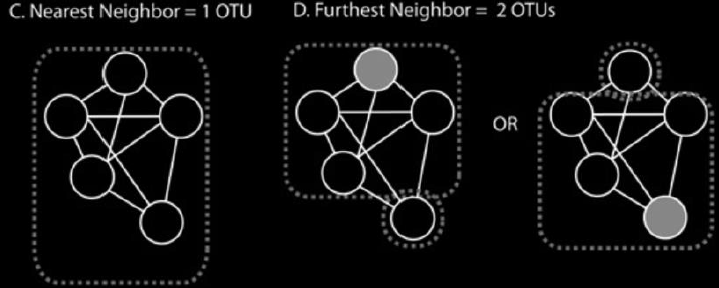
\includegraphics[width=0.9\textwidth]{overclustering.png}
      \caption{\label{fig:overclustering}Example of overclustering and result multiplicity due to complete linkage analysis}
    \end{figure}

  \subsection{OTU taxonomic annotation}
    \textbf{NOTE: this topic continues in the next lecture; when done merge together}
    Assigning a taxonomic annotation to an OTU cannot be done simply using BLAST to get the best matching sequence; this is because there is too much noise in the sequences and because it is difficult to classify new strains. A better way is using some other algorithm that assigns the terms of the taxonomic notation (since it is more than just one label) and provides some degree of confidence in the prediction. For instance the algorithm may be able to correctly assign the first taxonomical terms, up until \textit{Enterobacteriaceae}, but then it provides a prediction of the OTU belonging to \textit{E. coli} with some confidence interval, say 85\%, and some alternative like \textit{S. dysenteriae}, say with 15\% confidence.

\subsection{RDP classifier (Naive Bayes Model)}

P(S|G) is computed by RDP using a 8-mer strategy basically comparing the 8-mers in S with the 8-mers in all the training sequences available for genus G. The confidence of each prediction is computed by bootstrapping: 

\begin{itemize}
    \item Select a (random) subsequence of S, Say S’ 
    \item Compute the G that maximizes P(S’|G) 
    \item Repeat the procedure 100 times 
    \item The number of time G is selected by the bootstrapping procedure is the confidence 
\end{itemize}

Leave one-out-cross validation: 

\begin{itemize}
    \item Take out one data point from the training set
    \item Apply the classifier on the left-out point (without using it in the training set)
    \item Check the accuracy of the prediction
    \item Repeat the procedure for each training data point
\end{itemize}

The RDP classification accuracy is evaluated with the leave-one-out cross validation on the training set of hundreds thousands of 16S references: 

\begin{itemize}
    \item Accuracy $\xrightarrow[]{}$ percentage of correct classification (over the all leave-one-out runs)
    \item Varying levels of the taxonomic resolution (from phylum to genus)
    \item Varying sequence lengths
    \item In real applications accuracies are probably smaller:
    \begin{itemize}
        \item Sequencing errors
        \item "unknown bacteria"
    \end{itemize}

\end{itemize}

\section{Diversity analysis}

\begin{figure}[h]
\centering
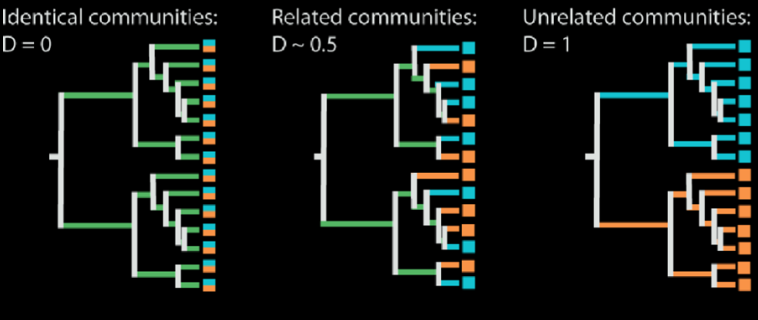
\includegraphics[width=0.6\textwidth]{UniFrac.png}
\caption{}
\end{figure}

\subsection{Alpha diversity analysis}

Alpha diversity analysis is a measure of how diverse, so complex, is a microbial community. "Within sample" diversity. Species richness is a widely use alpha diversity index. 
All individuals considered have non-zero abundance, some will have high abundance ($\sim$~99$\%$) or low abundance (1$\%$). High alpha diversity are usually associated with populations that are more robust and resilient to changes.
For examples gut microbiome with a high richness is usually associated with healthy state, instead of disease. 

\subsection{Beta diversity analysis}

Beta diversity analysis is a measure of how different two microbial communities are. "Between sample" diversity. It is possible to measure the beta-diversity using the inverse of number of shared species.
An example of beta-diversity is \textbf{UniFrac}. In UniFrac the distance is equal to the fraction of the total branch length that is unique to any particular environment. UniFrac can be also weighted in order to include abundances for each OTU.

\begin{figure}[h]
\centering
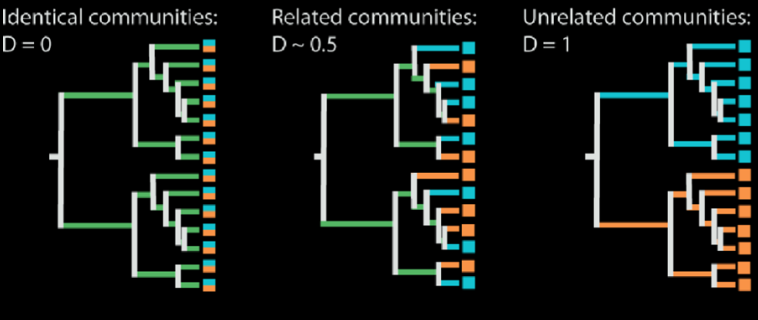
\includegraphics[width=0.6\textwidth]{UniFrac.png}
\caption{\textbf{D=0.} Blue and orange samples always have the same OTUs. Each 16S (each ramo) is present in both samples. \textbf{D=$\sim$0.5.}In reality we usually have a mix of the 2 situations. Some OTUs are present only in one of the samples and are either quite distant from the others or close (based on upstream the branch goes). \textbf{D=1.} Completely distinct OTUs . The difference is also in the upstream branches, which have different colors.}
\end{figure}

\section{Principal Coordinate Analysis (PCoA}

PCoA is also known as multidimensional scaling. It is one of the most powerful approaches for exploratory analysis. The idea is to represent the multidimensional relationship between samples in a two or three dimensional space. It is possible to use any similarity function as Euclidean distance, UniFrac, bray-Curtis distance. We find frequently hierarchical clustering plots. 

\section{Study: \textit{Enhanced microbial diversity in the saliva microbiome induced by short-term probiotic intake revealed by 16S rRNA sequencing on the IonTorrent PGM platform}}

The pool was made of 14 samples and some of them with probiotic administration, so a very small number of high-quality reads. The samples number 1 and 2 are of the same student that repeat the sampling twice in order to see the reproducibility of the technique.
All the students had firmicutes, proteobacteria and Bacteroidetes, plus a little bit of actinobacteria.

\begin{figure}[h]
\centering
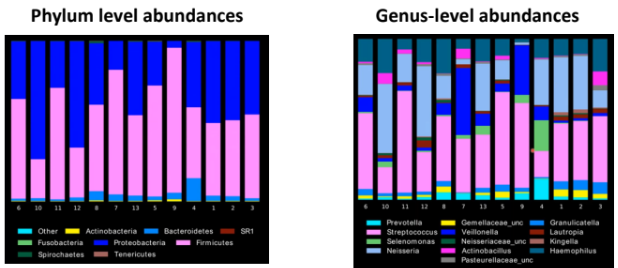
\includegraphics[width=0.6\textwidth]{Level.png}
\caption{}
\end{figure}

You cannot compare alpha-diversity of different student at different sequencing depth, but at the same.
When you do PCR, multiplexing and you put multiple samples on the same sequencing run the sequencing machine
will not get the exact n° of reads for each sample, you have a quite high variability. Since you cannot compare alpha-diversities at multiple sequencing depths, usually you have to decide a sequencing depth cut-off at least for alpha-diversity analysis. The greater the sequencing depth, the greater the alpha-diversity. 

\begin{figure}[h]
\centering
\includegraphics[width=0.6\textwidth]{AlphaDiversity.png}
\caption{\textbf{Alpha diversity and rarefaction plots.} The cut-off should not be too high, otherwise some samples will not be included in the further analysis. (If they do not reach depth, like the student 4 in light green.)}
\end{figure}

\begin{figure}[h]
\centering
\includegraphics[width=0.6\textwidth]{Probiotic.png}
\caption{\textbf{Probiotic effect on saliva microbiome?} Students that took the probiotic had a more diverse microbiome, and the maximum diversity was reached by taking probiotics at lunch.}
\end{figure}

\begin{figure}[h]
\centering
\includegraphics[width=0.6\textwidth]{Probiotic2.png}
\caption{\textbf{Is the effect due to the probiotic Streptococcus?} The probiotic product contained \emph{}{Streptococcus thermophilus}, \emph{}{Lactobacillus delbrueckii subsp. bulgaricus} and
\emph{Lactobacillus paracasei}. What if we remove OTUs from these genera from the dataset?The analysis is still significant. This means that the probiotics yogurt induces a variation in the microbiome that make it more diverse.}
\end{figure}

\begin{figure}[h]
\centering
\includegraphics[width=0.6\textwidth]{BetaDiversity.png}
\caption{\textbf{Looking at beta diversity} There is no clusters.}
\end{figure}

\chapter{Shotgun metagenomics}

\chapter{Staphylococcus aureus}


\end{document}
